%===========Kapitola: Impulzně regulované napájecí zdroje=========================================== 
\chapter{Impulzně regulované napájecí zdroje}
\minitoc
\newpage
  \section{Úvod}
    Spínané napájecí zdroje plní funkci stejnou jako zdroje se spojitou regulací. Vý\-ko\-no\-vý
    člen spínacích zdrojů je však zatěžován impulzně, tj. střídavě spínán a rozepínán. Lze tedy
    využít výhody impulzního režimu, tj. odebírat impulzní výkon podstatně větší, než je trvalý
    výkon při lineárním režimu regulátoru s týmž výkonovým členem. Spínací zdroje mají obecně větší
    účinnost než zdroje se spojitou regulací. Jsou výhodné zvláště tam, kde je velký rozdíl napětí
    na vstupu a výstupu regulátoru a kde jsou požadované malé rozměry. Impulzní regulace zajistí
    stabilizované výstupní napětí i pro velké změny vstupního napětí; účinnost zdroje se při tom
    téměř nemění. I přes větší obvodovou složitost jsou ekonomicky výhodnější, neboť jejich použití
    vede k podstatné energetické úspoře.
  
    Impulzně regulované zdroje však mají v porovnání se zdroji s lineární regulací i některé
    nevýhodné vlastnosti, například pomalejší reakci výstupního napětí na rychlé změny zatěžovacího
    výstupního proudu. Při požadavku malého zvlnění výstupního napětí se nesmí zanedbat vliv
    impulzního charakteru těchto zdrojů. Impulzně regulované zdroje jsou také zdrojem rušivých
    signálů, které jsou generovány spínacími prvky \cite[s.~112]{Hammembauer}.
       
    % \begin{table}[ht!]
      % \centering
      % \setlength{\tabcolsep}{5pt}
      % \begin{tabular}{p{1.2cm}p{7cm}}
        % \hline
        % \multirow{2}{*}{\googlepdflink{AN556}{https://docs.google.com/file/d/0BzP8spWKnOvnLXZBV3YzLWloR0U/edit}}
         % &  \textbf{Introduction to Power Supplies} \pdfcomment[icon=Note, color=Melon]{ahoj}\\
         % &  2002 National Semiconductor    \\
         % \hline
       % \end{tabular}
    % \end{table}    
   
  \section{Impulzní regulace ve výkonové elektronice}\label{ENZ:kap_Imp_Reg}
    Základním principem a současně odlišností impulzní regulace od regulace klasické je v její
    \emph{nespojitosti}. To znamená, že nehledě na detailní realizaci, je výstupní napětí 
    stabilizováno zásahy regulačního členu pouze v určitých, časově omezených intervalech. Podstata 
    regulačního členu (regulátoru) tedy spočívá v řízení vzájemných časových relací aktivního a 
    pasivního intervalu pracovního cyklu v závislosti na velikosti zesílené regulační odchylky.
    
    Akční člen je tedy řízen dvouhodnotovým signálem, mající význam \emph{zapnutí} nebo 
    \emph{vypnutí} výkonové součástky. Následující příklad demonstruje, jak lze tento signál 
    vytvořit pomocí \textbf{pulzně-šířkové modulace} v simulátoru \ltLtspiceSW. V simulacích 
    některých topologií spínaných zdrojů bude místo zdroje s lineárně narůstajícím výstupním napětím 
    viz obr. \ref{enz:fig_pwm_wave} použita regulační odchylka.
    
    \begin{figure}[ht!]
      \centering
      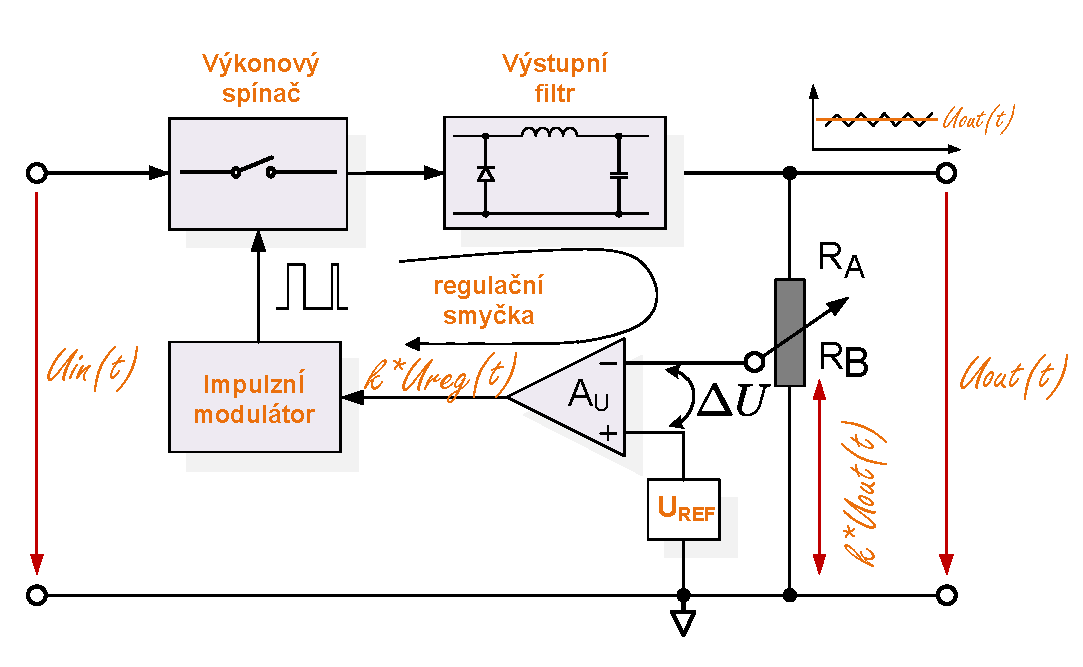
\includegraphics[width=\linewidth]{hamm_schema_imp_reg.pdf}
      \caption[Schéma impulzního regulátoru]{Základní schéma impulzního regulátoru}
      \label{enz:fig_imp_reg_basic}
    \end{figure}
    
    Srovnáme-li pro názornost klasický a impulzní regulátor na úrovni blokových schémat, vidíme, že 
    obě jsou formálně dosti podobná. U obou nacházíme napěťový normál \texttt{Uref}, zesilovač 
    regulační odchylky \texttt{Au}, budící obvod i výkonový regulační člen a samozřejmě i 
    zpětnovazební smyčku. Tím však, snad až na základní podstatu regulační smyčky podobnost končí. 
    Funkčně jsou oba regulátory naprosto odlišné.
    
    U spojitého lineárního regulátoru ovládá odchylka výstupního napětí od jmenovité velikosti 
    spojitě okamžitý odpor výkonového regulačního členu v libovolném o\-kam\-ži\-ku tak, aby 
    výstupní napětí bylo konstantní. Z toho, jak je již známo, vyplývá velká poměrná výkonová ztráta 
    na regulačním členu a tedy i malá účinnost spojité regulace za běžných provozních podmínek.
    
    Impulzní regulace obr. \ref{enz:fig_imp_reg_basic} umožňuje výrazně snížit výkonovou ztrátu na
    regulačním členu. V tomto případě pracuje regulační prvek (tranzistor) jako řízený spínač. Proud 
    jím tedy prochází pouze po určitý interval pracovního cyklu. Přitom okamžitá výkonová ztráta v 
    aktivním (sepnutém) stavu je vzhledem k $U_{CES}\rightarrow 0$ řádově menší, než u lineárního 
    regulátoru. Další předností je, že velikost ztráty v podstatě nezávisí na rozdílu vstupního a 
    výstupního napětí, ale prakticky pouze na kolektorovém proudu tranzistoru.
    
    Možnost použít spínací regulační člen při stabilizaci stejnosměrného napětí je podmíněna jeho 
    vzájemnou součinností s filtračním členem, který na rozdíl od aplikace ve spojitém regulátoru 
    musí mít výrazný akumulační charakter. Uspořádání filtru, který je pro větší výkony vždy typu 
    LC, je podřízeno topologii měniče. Princip činnosti nerozlučně vázané dvojice spínač - 
    akumulační výstupní filtr spočívá v akumulaci energie, která je v aktivním intervalu odebrána ze 
    zdroje, aby mohla být v následujícím pasivním intervalu (spínač vypnut) dodávána z filtru do 
    zátěže \cite[s.~121]{Hammembauer}.
           
    \begin{example} 
      Na obr. \ref{enz:fig_pwm_gen} je realizován generátor šířkově modulovaného signálu pro
      simulátor \texttt{LTSpice}, jenž s výhodou využívá komponenty \texttt{B-source}, umožňující
      behaviorální popis požadovaného průběhu.
      \begin{figure}[ht!]
        \centering
        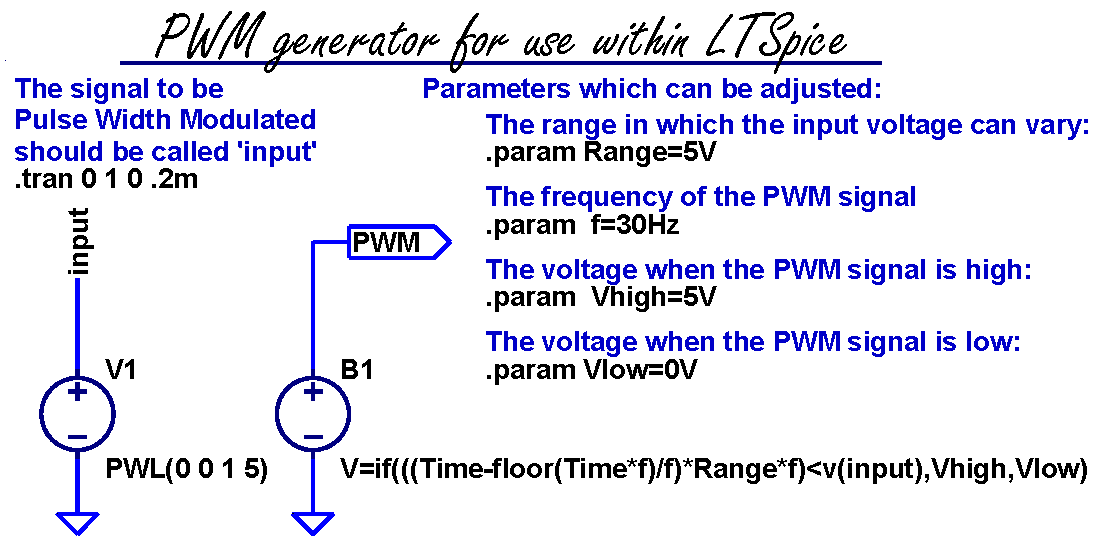
\includegraphics[width=\linewidth]{LTspice_pwm_gen.pdf}
        \caption[LTSpice - PWM generátor]{Realizace PWM generátoru pomocí komponenty B-source
                \emph{(Arbitrary behavioral voltage or current source)} v LTSpice (soubor
                \texttt{pwm.asc})}
        \label{enz:fig_pwm_gen}
      \end{figure}
      Podrobnějším pohledem na zápis rovnic dle obr. \ref{enz:fig_pwm_gen}, lze dojít k závěru, že
      zdroj \texttt{B1} na svůj výstup vnutí hodnotu parametru \texttt{Vhigh}, nebo \texttt{Vlow},
      podle výsledku rozhodovací funkce \texttt{if}. Tj. jeli
      \texttt{Time-floor(Time*f)/f)*Range*f)} větší než \texttt{V(input)}, bude na výstupu $V_{high}
      = 5V$, v opačném případě $V_{low} = 0V$. Funkce \texttt{floor} zaokrouhluje hodnotu svého
      argumentu na celé číslo (\texttt{integer}), což vede na schodovitý průběh a funkce
      \texttt{Time} umožňuje do vztahu vnést okamžitou hodnotu simulačního času. Vzájemný odečtením
      získáme pilový průběh, kterým se komparuje s okamžitou hodnotou zdroje \texttt{V(input)}.
       
       \begin{figure}[ht!]
         \centering
         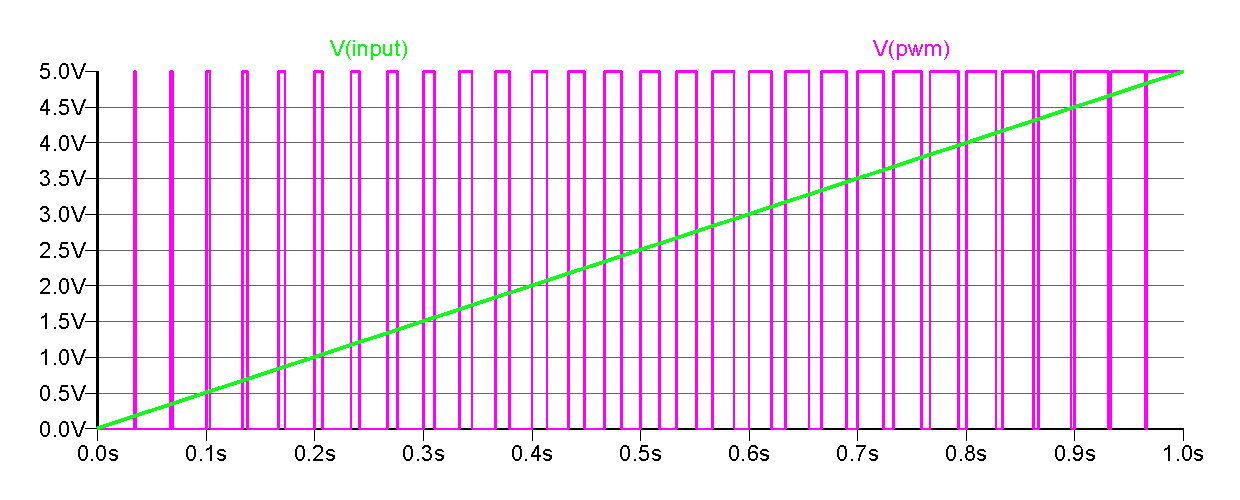
\includegraphics[width=1\linewidth]{LTspice_pwm_wave.pdf}
         \caption[LTSpice - PWM generátor: průběhy]{Výstupní signál \texttt{V(pwm)} z PWM
                  generátoru na obr. \ref{enz:fig_pwm_gen}  má-li rozhodovací napětí \texttt{V(in)}
                  lineární charakter}
         \label{enz:fig_pwm_wave}
       \end{figure}       
    \end{example} 
   
    \newpage
    %------------------------------------------------------
    % Section: DC/DC měniče s transformátorem
      % DC_DC_converter.tex
%===============================Podkapitola: DC/DC měniče bez transformátoru========================
  \section{DC/DC měniče bez transformátoru}\label{ENZ:kap_DC_DC}
    \subsection{Vymezení pojmů a základních požadavků}
      DC - DC měniče jsou obvody sloužící k regulaci elektrické energie, které mění vstupní
      stejnosměrně napětí U1 na jiné výstupní stejnosměrné napětí U2. Budeme se přitom zabývat
      měniči tzv. \emph{napěťového typu}, což jsou měniče napájené konstantním vstupním napětím z
      napěťového zdroje, nikoliv proudem, z proudového zdroje. V této kapitole se omezíme pouze na
      měniče bez transformátoru, které tedy neumožňuji galvanické oddělení výstupu od vstupu
      \cite{Patocka}.

      Každý měnič sestává z vlastního silového obvodu a řídicí elektroniky (regulačních obvodů).
      Silové obvody nesmí využívat při regulaci energie rezistorů a proto se mohou skládat jen ze
      \textbf{spínačů} a \textbf{akumulačních prvků}, tj. \emph{indukčnosti} a \emph{kapacit}.

      \subsubsection{Napájecí zdroj a zátěž měniče}
        \begin{figure}[b]
          \centering
          \subfloat[náhradní schéma akumulátoru]{\label{enz:fig_nahr_sch_aku}
            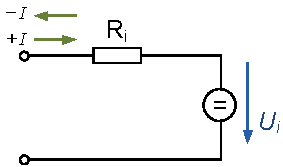
\includegraphics[width=0.4\linewidth]{patocka_aktivni_zatez_nahrad_sch.pdf}}
           \hfill 
           \subfloat[náhradní schéma stejnosměrného elektromotoru s cizím
                     buzením]{\label{enz:fig_nahr_sch_ss_motor}
            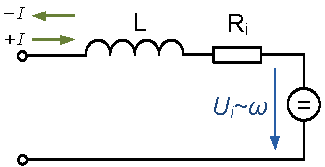
\includegraphics[width=0.4\linewidth]{patocka_aktivni_zatez_ss_mot_nahrad_sch.pdf}}
          \caption{Aktivní zátěž.}
          \label{enz:fig_aktivni_zatez}
        \end{figure}
        DC/DC měniče mohou přenášet energii z principu oběma směry. Mohou tedy čerpat energii ze
        zdroje a dodávat ji do zátěže nebo také opačně energii čerpat ze zátěže a dodávat ji do
        zdroje. Pojmy zátěž a zdroj je proto nutné chápat v širším slova smyslu.
        \begin{itemize}
          \item Zdrojem s konstantním napětím $U_1$, schopným dodávat i akumulovat energii, je
                akumulátor. Použijeme-li jako zdroj např. usměrňovač se sběrným kondenzátorem, pak
                není schopen dlouhodobě jímat energii z měniče, tj. dlouhodobě nesmí ve střední
                hodnotě převládat směr proudu do kladné svorky zdroje (krátkodobě, v okamžité
                hodnotě, je takový směr možný). Nabíjením sběrného kondenzátoru by totiž rostlo
                napětí $U_1$. Tomu lze zabránit přeměnou dodávané energie na teplo ve vybíjecím
                rezistoru, či na Zenerově diodě, zapojené paralelně ke sběrnému kondenzátoru.
          \item Z hlediska schopnosti spotřeby či dodávky energie, lze rozlišovat zátěž
                \emph{aktivní} a \emph{pasivní}. Aktivní zátěži je opět např. akumulátor, ale třeba
                i stejnosměrný motor. Jeho náhradní zapojeni, platné v ustáleném stavu, je uvedeno
                na obr. 1 1). Vnitřní rotační (pohybové) indukované napětí je úměrně otáčkám, proud
                pak momentu na hřídeli a to včetně znamének.
        \end{itemize}

        Teče-li proud ve  střední hodnotě do zátěže (+I), pak motor pohání, tj. mění elektrickou
        energii na mechanickou (pracuje v \emph{motorickém režimu}). Teče-li ze zátěže (-I), pak
        motor brzdí, tj. mění z vnějšku dodávanou mechanickou energii na energii elektrickou
       (pracuje v \emph{generátorickém režimu}).
       
      \subsubsection{Pracovní kvadranty}
         \begin{figure}[ht!]
           \centering
           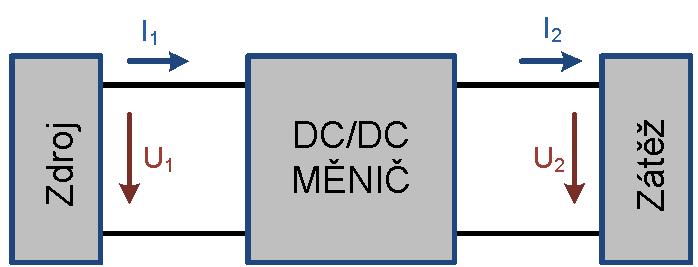
\includegraphics[width=0.7\linewidth]{patocka_pracovni_kvadranty_sch.pdf}
           \caption{Označení vstupních a výstupních veličin DC/DC měniče.}
           \label{enz:fig_prac_kvadranty_sch}
         \end{figure}

         Označme si vstupní a výstupní napětí a proud měniče podle obr.
         \ref{enz:fig_prac_kvadranty_sch}. Podle polarity výstupního napětí $U_2$ a výstupního
         proudu $I_2$ může měnič pracovat ve čtyřech kvadrantech tzv.\textbf{ VA-roviny} (viz obr.
         \ref{enz:fig_prac_kvadranty}).

         V kvadrantech \emph{1} i \emph{3} dodává měnič energii do zátěže. Je-li zátěží motor, tak
         pohání. Pasivní zátěže mohou pracovat pouze v těchto kvadrantech. V kvadrantech \emph{2} a
         \emph{4} dodává aktivní zátěž energii zpět do měniče. Jde-li o motor\footnote{Velikost
         napětí ss. motoru je úměrná otáčkám (rychlosti), polarita je dána směrem otáčení
         (uvažujeme motor s cizím buzením, např. s permanentními magnety). Velikost proudu je
         úměrná momentu na hřídeli, polarita je opět dána směrem momentu, tj. zda motor brzdí či
         pohání. Je třeba si povšimnout, že přechod mezi generátorickým a motorickým režimem mezi
         kvadranty 2 a 1 nebo mezi 3 a 4 (tj. takový, kdy se nemění polarita napětí, ale jen
         proudu) vůbec nemusí být na hřídeli motoru opticky pozorovatelný, neboť v dané chvíli
         přechodu se změní jen znaménko momentu (proudu) a přesto otáčky hřídele mohou být
         konstantní.}, pak brzdí.

      \subsubsection{Možnosti zapojení silového obvodu}\label{enz_kap_moznosti_zapojeni}
         \begin{figure}
           \centering
           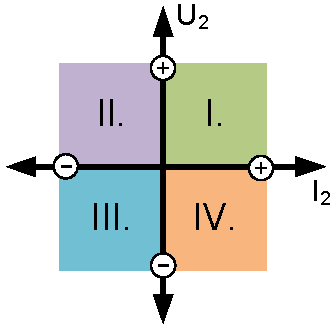
\includegraphics[width=0.5\linewidth]{patocka_pracovni_kvadranty.pdf}
           \caption{Pracovní kvadranty ve VA rovině.}
           \label{enz:fig_prac_kvadranty}
         \end{figure}
         Na první pohled jsou zřejmá určitá omezení:
         \begin{itemize}
       	   \item Indukčnost nikdy nesmí být zapojena paralelně ke vstupu či výstupu (protože tam je
                 napětí s nenulovou střední hodnotou).
           \item Kapacita nikdy nesmí být zapojena do série se vstupní nebo výstupní svorkou měniče
                 (protože tudy prochází proud s nenulovou střední hodnotou).
           \item Jako akumulační prvek nelze použít samostatně kapacitu, není-li v obvodu použita
                 ještě indukčnost (protože by v měniči napěťového typu docházelo k nepřípustnému
                 nárazovému nabíjení kondenzátoru zkratovým proudem). Čili měnič napěťového typu
                 musí obsahovat alespoň jednu indukčnost.
           \item Žádný spínač nesmí zkratovat vstup ani výstup měniče.
         \end{itemize}
      \subsubsection{Nejjednodušší měniče s jediným akumulačním 
                     prvkem}\label{ENZ:tit_menice_s_1_aku_prvkem} 
         Pro výchozí představu, vysvětlující princip činnosti, vytvoříme silový obvod měniče ze
         dvou prvků. Bude to indukčnost  \emph{L} a ideální přepínač. Vezmeme-li v úvahu omezení z
         kap. \ref{enz_kap_moznosti_zapojeni}, existují podle obr. \ref{enz:fig_DCDC_princip} jen
         tři způsoby, jak takový měnič zapojit \cite{Patocka}.

        \begin{figure}[ht!]
          \centering
          \begin{tabular}{c}
            \subfloat[$U_x=U_1\frac{t_1}{t_1+t_2}<U_1$]{\label{enz:fig_stepdown}
              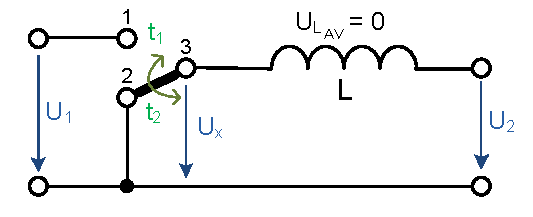
\includegraphics[width=0.8\linewidth]{patocka_step_down_princip.pdf}}     \\
            \subfloat[$U_x=U_2\frac{t_1}{t_1+t_2}>U_1$]{\label{enz:fig_stepup}
              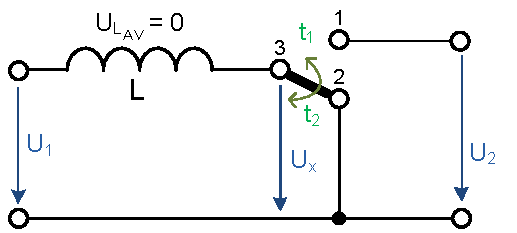
\includegraphics[width=0.8\linewidth]{patocka_step_up_princip.pdf}}       \\
            \subfloat[$U_x=\frac{U_1\cdot t_1 + U_2\cdot
                      t_2}{t_1+t_2}<>-U_1$]{\label{enz:fig_buckboost}
              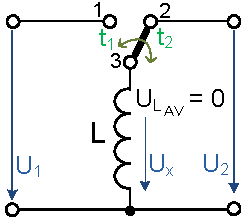
\includegraphics[width=0.7\linewidth]{patocka_buck_boost_princip.pdf}}
          \end{tabular}  
          \caption{Principiální schémata DC/DC měničů s jediným akumulačním prvkem.}
          \label{enz:fig_DCDC_princip}
        \end{figure}

        Označme střední hodnotu napětí mezi společným uzlem přepínače \texttt{3} a zemí jako 
        $U_x$. Předpokládejme, že přepínač je ovládán periodickým signálem s periodou $T$ a s
        nastavitelnou střídou, takže po dobu  $t_1$ spojuje svorky \texttt{3 - 1} a po dobu  $t_2 =
        T – t_1$ pak svorky \texttt{3 - 2}. Popišme nyní nejzákladnější vlastnosti tří měničů z
        obr. \ref{enz:fig_DCDC_princip}.

        \begin{enumerate}
          \item Střední hodnota $U_x$ na obr.\ref{enz:fig_stepdown} musí vzhledem k činnosti
                přepínače být:
                \begin{equation}\label{enz:stepdown_Ux}
                  U_x = U_1\frac{t_1}{t_1 + t_2} < U_1
                \end{equation}
                Výstupní napětí je rovno $U_x$, neboť střední hodnota napětí na indukčnosti L musí
                být nulová. Platí proto:
                \begin{equation}\label{enz:stepdown_U2}
                  U_2 = U_x = U_1\frac{t_1}{t_1 + t_2} < U_1
                \end{equation}
                Výstupní napětí je vždy menší než vstupní a má stejnou polaritu. Jde tedy o měnič
                \emph{snižující} a \emph{neinvertující}. Jeho jiné názvy jsou: \textbf{step-down,
                chopper, buck, propustný měnič}. Možné pracovní kvadranty jsou 1 a 2. Čili měnič je
                schopen dávat napětí $U_2$ jediné polarity, ale proud $I_2$ muže téci oběma směry
                (je-li to umožněno - aktivní zátěž).
          \item Střední hodnota $U_x$ na obr.\ref{enz:fig_stepup} musí vzhledem k činnosti
                přepínače být:               
                \begin{equation}\label{enz:stepup_Ux} 
                  U_x = U_2\frac{t_1}{t_1 + t_2} > U_1
                \end{equation}
                Vstupní napětí $U_1$ je rovno $U_x$ (nulová střední hodnota napětí na indukčnosti
                L). Odsud pro $U_2$ platí:
                \begin{equation}\label{enz:stepup_U2}
                  U_2 = U_1\frac{t_1 + t_2}{t_1} > U_1
                \end{equation}
                Střední hodnota výstupního napětí je vyšší než vstupní napětí a má stejnou polaritu.
                Jde tedy o \emph{zvyšující} a \emph{neinvertující} měnič. Jiný název je měnič
                \textbf{step-up, boost}. Možné pracovní kvadranty\footnote{Měnič
                \ref{enz:fig_stepdown} pracující v kvadrantu 1 je měničem \ref{enz:fig_stepup}
                pracujícím v kvadrantu 2. Naopak \ref{enz:fig_stepdown} v kvadrantu 2 je
                \ref{enz:fig_stepup} v kvadrantu 1. Čili \ref{enz:fig_stepdown} a
                \ref{enz:fig_stepup} je vlastně týž obvod, pouze zaměňuje vstup a výstup.} jsou opět
                1 a 2.
          \item Střední hodnota $U_x$ na obr.\ref{enz:fig_buckboost} musí vzhledem k činnosti
                přepínače být:
                \begin{equation}\label{enz:buckboost_Ux}
                  U_x = \frac{U_1t_1 + U_2t_2}{t_1 + t_2} <> - U_1
                \end{equation}
                Protože $U_x$ je střední hodnota napětí na indukčnosti L, musí platit $U_x =0$ tj.
                \begin{equation}\label{enz:buckboost_U2}
                  U_1 = - \frac{t_1}{t_2}U_1 <> - U_1
                \end{equation}
                Výstupní napětí má opačnou polaritu než vstupní, jde tedy o měnič
                \emph{invertující}. Velikost výstupního napětí může být větší i menší než vstupní.
                Vžité názvy jsou měnič \textbf{buck-boost, měnič se společnou tlumivkou, blokující
                měnič}. Možné pracovní kvadranty jsou 3 a 4.
        \end{enumerate}

      \subsubsection{Prakticky realizované silové obvody}\label{ENZ:subkap_silove_obvody}
        Kap. \ref{ENZ:tit_menice_s_1_aku_prvkem} ukazuje, že elektronicky ovládaný přepínač tvoří
        základní stavební kámen každého měniče. Tyto přepínače se ve skutečných obvodech realizují
        pomocí tzv. horních a dolních spínačů, což jsou \emph{trojpóly} podle obr.
        \ref{enz:fig_silove_obvody}.
        \begin{figure}
          \centering
          \begin{tabular}{c}
            \subfloat[Horní spínač]{\label{enz:fig_HS}
              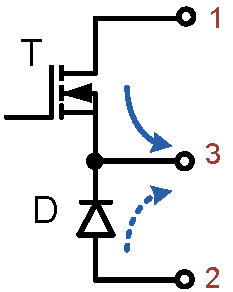
\includegraphics[width=0.3\linewidth]{patocka_horni_spinac.pdf}}     \\
            \subfloat[dolní spínač]{\label{enz:fig_LS}
              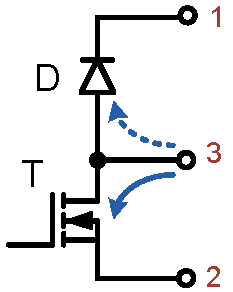
\includegraphics[width=0.3\linewidth]{patocka_dolni_spinac.pdf}}     \\ 
            \subfloat[Větev - paralelní kombinace horního a dolního spínače]{\label{enz:fig_arm}
              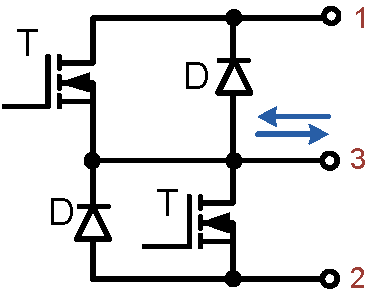
\includegraphics[width=0.4\linewidth]{patocka_vetev.pdf}}
          \end{tabular}  
          \caption{Horní a dolní spínač.}
          \label{enz:fig_silove_obvody}
        \end{figure}

        \begin{figure*}
          \centering
          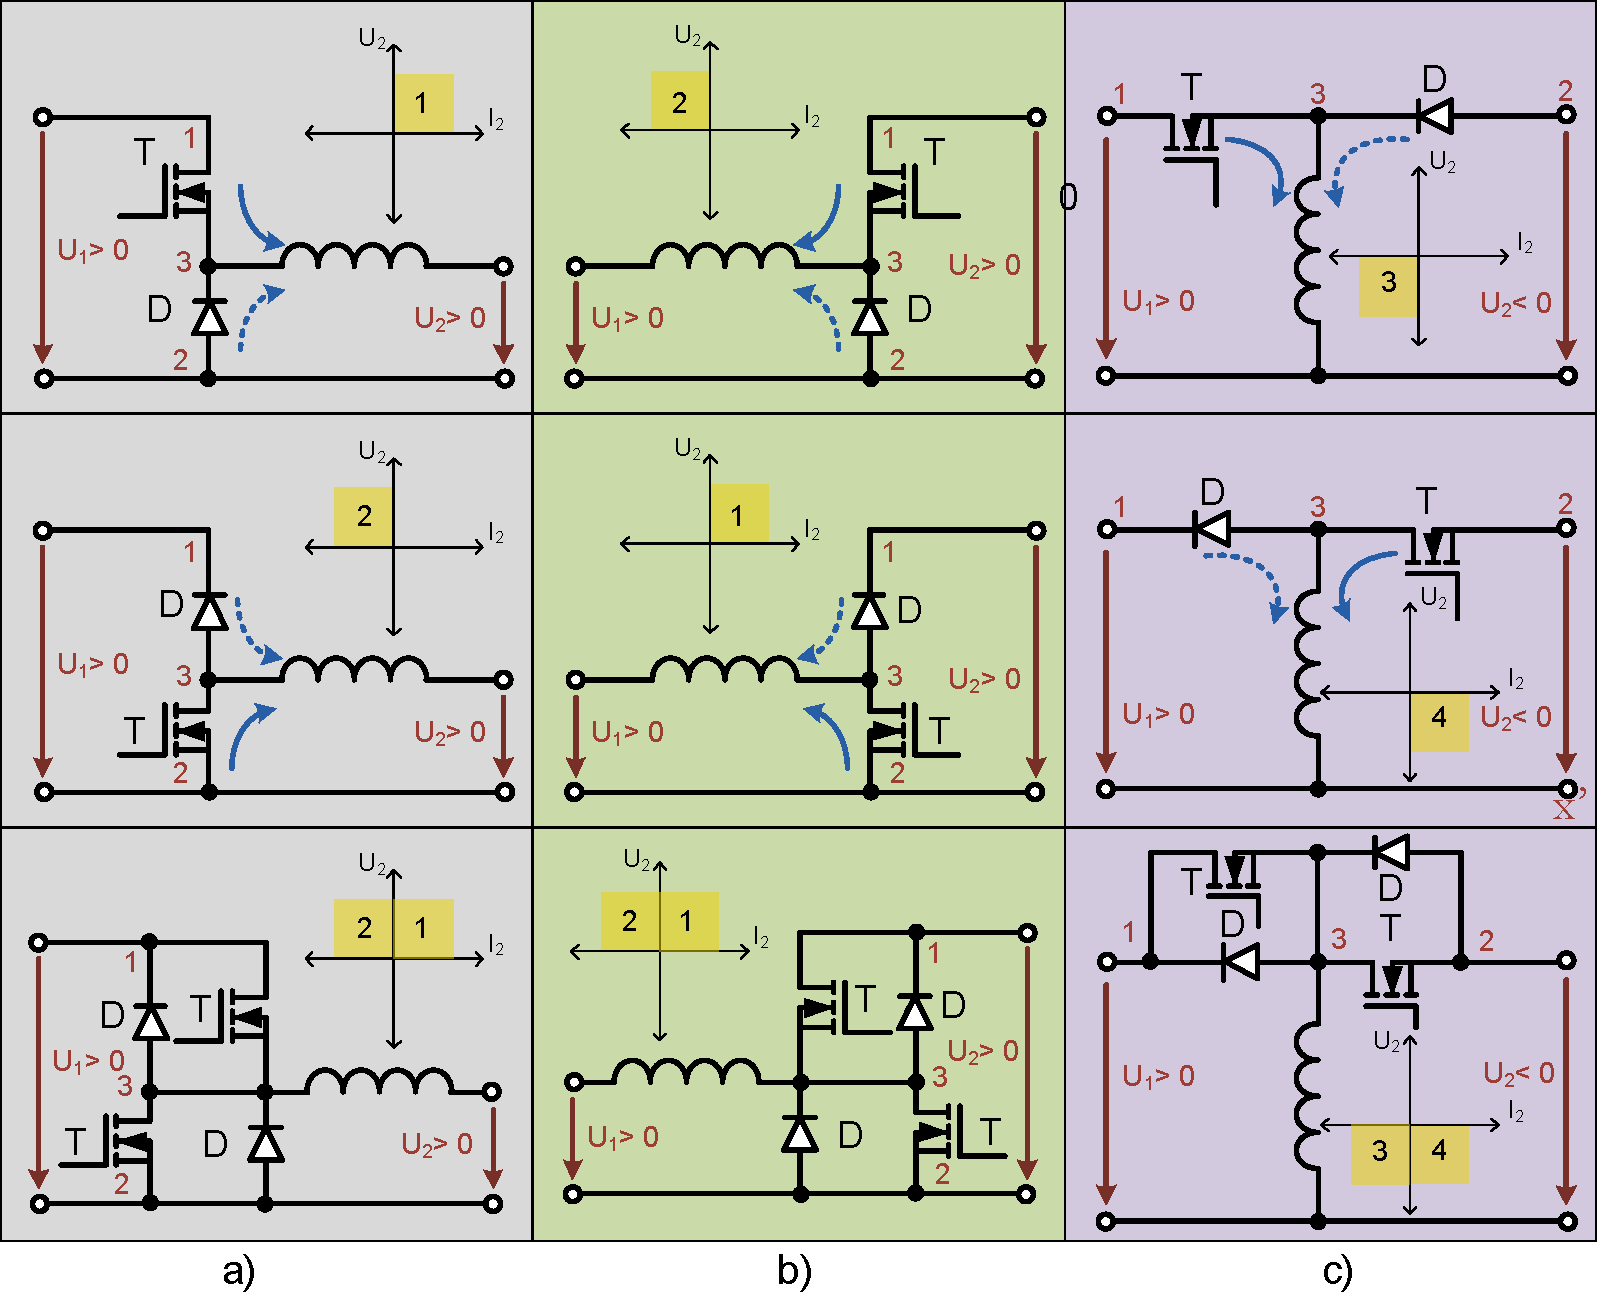
\includegraphics[width=0.9\textwidth]{patocka_silove_obvody_kvadranty.pdf}
          \caption[Skutečné silové obvody měničů a jejich kvadranty]{Skutečné silové obvody měničů
                   z obr. \ref{enz:fig_DCDC_princip} a jejich pracovní kvadranty: a) měnič snižující
                   neinvertující (step-down), b) měnič zvyšující neinvertující (step-up), c) měnič
                   invertující (buck-boost)}
          \label{enz:fig_silove_obv_kvadranty}
        \end{figure*}
        
\subsection{Step-down converter \newline(snižující neinvertující měnič)}\label{ENZ:kap_step_down}
  Jedná se o měnič s horním spínačem. Další jeho používané názvy jsou: propustný měnič, chopper,
  buck. \emph{Pracuje v 1. kvadrantu}.
  \begin{figure}[ht!]
    \centering
    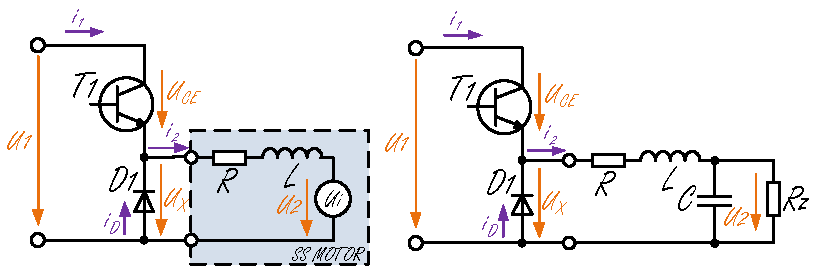
\includegraphics[width=1\linewidth]{patocka_step_down_sch1.pdf}
    \caption[Snižující měnič]{Snižující měnič pracující v prvním kvadrantu s aktivní zátěží
             typu stejnosměrný motor nebo s LC filtrem}
    \label{enz:fig_StepDown_sch1}
  \end{figure}

  \begin{figure}[ht!]
    \centering
    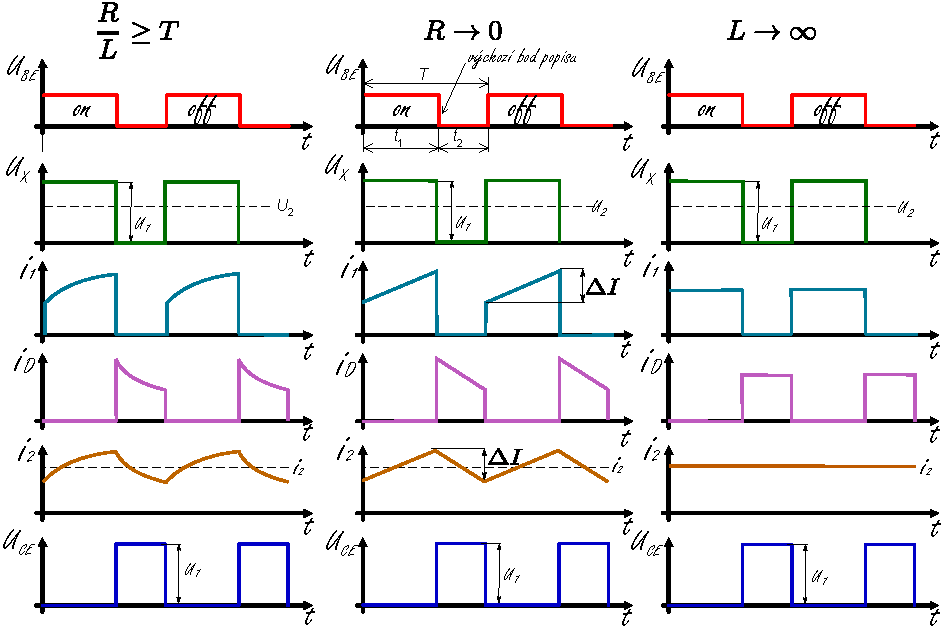
\includegraphics[width=1\linewidth]{patocka_step_down_waveform.pdf}
    \caption[Snižující měnič - průběhy]{Průběhy napětí a proudů snižujícího měniče}
    \label{enz:fig_StepDown_wave1}
  \end{figure}

\subsection{Step-up converter (zvyšující neinvertující měnič)}\label{ENZ:kap_step_up}
  \begin{figure}[ht!]
    \centering
    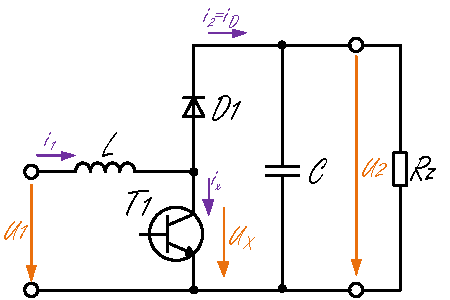
\includegraphics[width=0.8\linewidth]{patocka_step_up_sch1.pdf}
    \caption[Zvyšující měnič]{Zvyšujícího měnič pracující v prvním kvadrantu - Schéma zapojení}
    \label{enz:fig_StepUp_sch1}
  \end{figure}

\subsection{Buck-boost converter \newline(Invertující měnič se společnou tlumivkou)}\label{ENZ:kap_buck_boost}
\subsection{Cuk converter \newline(Měnič se společným konden\-zá\-to\-rem)}\label{ENZ:kap_cuk}
\subsection{SEPIC converter \newline(Single-ended primary inductor converter)}\label{ENZ:kap_sepic}         
    %------------------------------------------------------
    \newpage
    %------------------------------------------------------
    % Section: DC/DC měniče s transformátorem
      %======================= Podkapitola: DC/DC měniče s transformátorem ===============================
\section{DC/DC měniče s transformátorem}
  Základní popis DC/DC měničů bez transformátoru, provedený v kap. \ref{ENZ:kap_DC_DC}, platí i pro 
  měniče s transformátorem. Doplněním vhodně zapojeného vf. impulsního transformátoru je umožněno 
  galvanické oddělení výstupního a vstupního napětí a transformaci napětí a proudů. Nejčastěji se v 
  praxi setkáme s transformátorovými verzemi měniče propustného z kap. \ref{ENZ:kap_step_down} a 
  měniče blokujícího z kap.\ref{ENZ:kap_step_up} Existuje i transformátorová verze měniče Čukova z 
  kap. \ref{ENZ:kap_cuk}.

  Snižující měnič z kap \ref{ENZ:kap_step_down} je v transformátorové verzi nazýván výhradně jako
  \textbf{měnič propustný}, neboť díky transformátoru lze převodovým poměrem zajistit výstupní 
  napětí i vyšší než vstupní (názvy „\emph{snižující měnič}“ a „\emph{step-down}“ by tedy byly 
  zavádějící). Princip činnosti však v hrubých rysech zůstává stejný.

  Invertující měnič se společnou tlumivkou z kap. \ref{ENZ:kap_buck_boost} je v transformátorové 
  verzi nazýván výhradně jako \textbf{měnič blokující}, neboť díky transformátoru lze vyrobit napětí 
  libovolné polarity (název „\emph{invertující měnič}“ proto pozbývá výstižnosti).

  Základní stavební kameny měničů bez transformátoru tj. horní spínač a dolní spínač (kap.
  \ref{ENZ:subkap_silove_obvody}) tvoří základ i u měničů s transformátorem, i když v zapojeních 
  jsou tranzistor a jeho protilehlá dioda \emph{rozděleny} tím, že je tranzistor na primární straně 
  a dioda na sekundární. Použití transformátoru navíc vyžaduje demagnetizační obvody (zajištění 
  nulové střední hodnoty primárního napětí) a další výstupní usměrňovací diodu (diody). To vše vede 
  k tomu, že transformátorové měniče jsou \emph{jednokvadrantové}. Výstupní napětí má jedinou možnou 
  polaritu a výstupní proud jediný možný směr takový, že zátěž se chová vždy jako spotřebič, nikoli 
  jako generátor.

  %--------------- Jednočinný propustný měnič s impulsním transformátorem --------------------------
  \subsection{Jednočinný propustný měnič s impulsním transformátorem} 
    Propustné měniče se vyznačují tím, že energie je přenášena ze vstupu na výstup v době zapnutí 
    tranzistoru, nikoli v době vypnutí, jak je tomu u měničů blokujících.
    
    V této i v následujících kapitolách budou analyzovány měniče typu DC/DC, které obsahují 
    vysokofrekvenční impulzní transformátor na feritovém jádře. Transformátor zajišťuje galvanické 
    oddělení mezi vstupní a výstupní stranou měniče. Je-li vstupní stejnosměrné napětí získáno 
    usměrněním střídavé sítě, pak bývají tyto měniče někdy označovány jako tzv. \emph{síťové spínané 
    zdroje}.
    
    Celý výkonový řetězec sestává z následujících základních bloků:
    \begin{itemize}
      \item buď síťový usměrňovač - stejnosměrný meziobvod — vlastní měnič,
      \item nebo akumulátor — stejnosměrný meziobvod - vlastní měnič.
    \end{itemize}
    
    Stejnosměrný meziobvod (ss. mezilehlý obvod, DC-bus, zwischenkreis) bývá napěťového typu, tj. 
    vůči následujícímu měniči se chová jako (téměř) ideální zdroj konstantního napětí \(U_d\) 
    nulovou vnitřní impedancí. Bývá realizován buď LC-filtrem, nebo samostatným sběracím 
    kondenzátorem o velké kapacitě. Dvojcestným usměrněním sítě 1 x \SI{230}{\volt} vznikne na 
    sběracím kondenzátoru ss. mezilehlé napětí \(U_d\) o hladině přibližně \SI{300}{\volt}. 
    Šestipulsním usměrněním sítě 3 x \SI{400}{\volt} vznikne ss. napětí o jmenovité střední hodnotě 
    \SI{542}{\volt}.
    
    Na hladině \SI{542}{\volt} se obvykle používají tranzistory IGBT se závěrným napětím 
    \SI{1200}{\volt}, které pracují na spínacím kmitočtu od \SI{25}{\kilo\hertz} do 
    \SI{60}{\kilo\hertz} (podle přenášeného výkonu). Kmitočet je ve většině případů omezen především 
    přepínacími ztrátami v tranzistorech IGBT.
    
    Na hladině \SI{300}{\volt} bývají převážně používány tranzistory MOSFET se závěrným napětím 
    \SI{600}{\volt}. Tranzistory jsou v současnosti tak rychlé, že mohou pracovat na spínacím 
    kmitočtu až do \SI{300}{\kilo\hertz}. Pracovní kmitočet ležívá typicky v oblasti 
    \SI{40}{\kilo\hertz} až \SI{120}{\kilo\hertz}. Jediným důvodem ke zvyšování kmitočtu je 
    zmenšování objemu transformátoru i výstupní tlumivky. Zvyšování kmitočtu nad 
    \SI{200}{\kilo\hertz} není výhodné z následujících důvodů:
    \begin{itemize}
      \item Mezní kmitočet manganato-zinečnatých feritů leží kolem \SI{450}{\kilo\hertz}, tudíž 
            v pásmu nad \SI{200}{\kilo\hertz} prudce rostou hysterezní ztráty (viz komplexní 
            permeabilita v kap. 6.4.4.). Ztráty je nutno omezovat snižováním maximální pracovní 
            indukce \(B_{max}\), což působí proti zmenšování transformátoru.
       \item V oblasti nad \SI{200}{\kilo\hertz} začínají narůstat problémy se skinefektem ve vinutí 
            transformátoru (nikoli ve vinutí tlumivky, v ní je proud téměř hladký). Na kmitočtu 
            \SI{200}{\kilo\hertz} činí hloubka vniku již pouze \(\delta\cong\) \SI{0,14}{\mm}, viz 
            kap. 4. Nutné je použití vf. lanka nejen na sekundám (málo závitů a velký průřez), ale i 
            na primáni (více závitů a menší průřez). Výsledkem je pokles činitele plnění ve vinutí, 
            který působí proti zmenšování transformátoru.
      \item S rostoucím pracovním kmitočtem/dramaticky roste reaktance \(2\pi f L_{2,K}\) 
            výstupní rozptylové indukčnosti transformátoru \(L_{2,K} = L2(1 - k^2)\). Transformátor 
            je pak velmi měkký a není schopen přenést požadovaný výkon. Jedinou obranou je dosažení 
            co největšího činitele vazby \(k\). Hodnota \(k = 0,990\) je naprosto nedostatečná. 
            Nutným minimem bývá \(k = 0,998\), což ale přináší značné konstrukční problémy (viz kap. 
            17.6).
      \item S rostoucím kmitočtem roste negativní vliv parazitních mezizávitových kapacit vinutí.
    \end{itemize}
    
    %------------- Jednočinný propustný měnič - základní zapojení ----------------------------------
    \subsubsection{Jednočinný propustný měnič - základní zapojení}
      Základní zapojení jednočinného propustného měniče s transformátorem je nakresleno na obr. 
      \ref{enz:fig_fey_1cinprop_m}. Jak již bylo předesláno, k přenosu energie ze vstupního do 
      výstupního obvodu dochází v aktivním intervalu \(0\) až \(\delta T\), během něhož se současně 
      akumuluje energie v magnetickém poli tlumivky \(L\). Po dobu zbývající části periody 
      $(1-\delta)T$ je tlumivka od transformátoru oddělena a na výstup dodává energii nahromaděnou v 
      magnetickém poli. Vzhledem k \emph{blokujícímu měniči} je zde výhoda účinného LC filtru 
      tvořeného tlumivkou a výstupním kondenzátorem \(C\) po dobu celého pracovního cyklu. Ve 
      srovnání s blokujícím měničem je tedy možné dosáhnout řádově menší dynamické odchylky \(\Delta 
      U_z(t)\). Navíc proud tekoucí \(L\), skládající se z ustálené složky $I_z$ a pilovitého 
      průběhu $\Delta i_L$ má spojitý charakter v průběhu celé periody $T$. 
      
      Časové průběhy všech důležitých veličin jsou zachyceny na obr. \ref{enz:fig_fey_1cinprop_mw}. 
      Z důvodu snadnějšího výkladu budeme při prvotní analýze předpokládat následující zjednodušení:
  
      \begin{itemize}
        \item Tlumivka výstupního LC-filtru má velikou (nekonečnou) indukčnost. Proud tlumivky  
              \(i_L\) je hladký, málo zvlněný, tudíž je přímo roven proudu zátěže: \(i_L(t) = I_Z = 
              \text{konst}\).
        \item Transformátor má dokonalou magnetickou vazbu \(k=1\). Neexistuje tedy výstupní 
              rozptylová indukčnost \(L_{2,K}\).
      \end{itemize}
      Obě zjednodušení později při detailní analýze odstraníme.
      
      \begin{figure}
        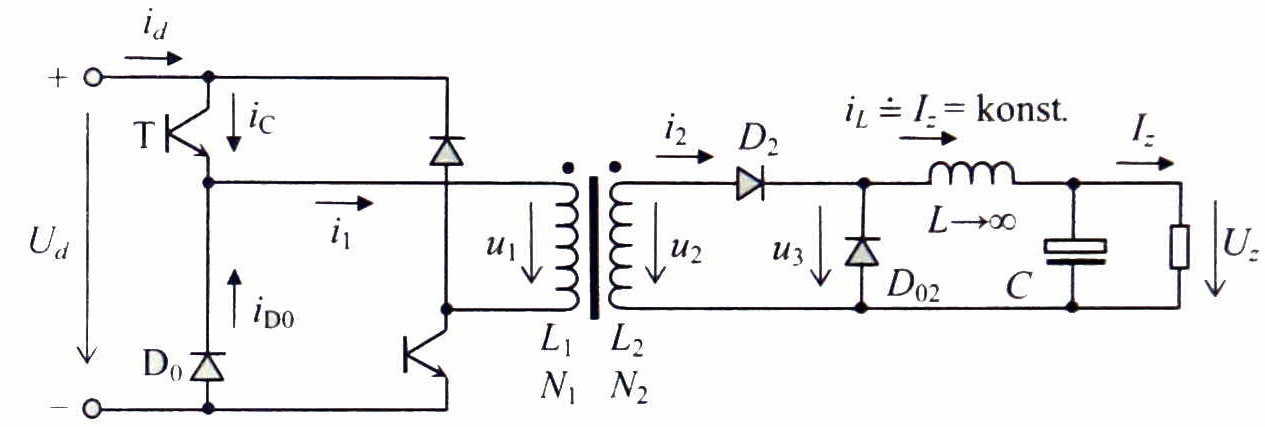
\includegraphics[width=\linewidth]{patocka_1cinprop_menic.JPG}
        \caption{Jednočinný propustný měnič - základní zapojení}
        \label{enz:fig_fey_1cinprop_m}
      \end{figure}
    
      Měnič pracuje tak, že oba tranzistory jsou vždy zapínány i vypínány současně. Doba zapnutí je označena
      \(t_z\). Střída je definována vztahem
      \begin{equation}\label{enz:eq_1cinpropm01}
        s = \frac{t_z}{T}, \qquad s_{max} = \frac{1}{2}, \qquad \text{protože} \qquad t<\frac{T}{2}
      \end{equation}     
  
      Maximální doba zapnutí \(t_z=t_1\), nesmí překročit hodnotu \(\dfrac{T}{2}\), neboť pak 
      dochází k lavinovitému přesycení transformátoru podle obr. \ref{enz:fig_fey_1cinprop_syc}. Při 
      zapnutí obou tranzistorů má primární napětí konstantní hodnotu \(U_1(t)=+U_d\). Magnetizační 
      proud je integrálem z tohoto \emph{konstantního} napětí, proto narůstá \emph{lineárně} (pokud 
      zanedbáme nelinearitu magnetizační charakteristiky). V okamžiku \(t_1\) jsou oba tranzistory 
      vypnuty. Magnetizační indukčnost \(L_1\), však nedovolí zánik magnetizačního proudu a snaží se 
      jej udržet na původní velikosti. Proud tedy musí začít téci oběma primárními diodami. Přes obě 
      sepnuté diody připojí primární vinutí samo sebe na napájecí zdroj \(U_d\) ale v opačné 
      polaritě, tedy bude \(U_1(t)=-U_d\). Tímto napětím je jádro \emph{demagnetováno} a 
      magnetizační proud klesá, protože integrál ze záporné konstanty je klesající přímka. Obě diody 
      se uzavřou až v okamžiku zániku magnetizačního proudu. Teprve tehdy je primární vinutí zcela 
      odpojeno od mezilehlého zdroje \(U_d\), stává se neutrálním vodičem neobsahujícím energii, 
      proto teprve tehdy klesne primární napětí na nulu.
      
      Sekundární napětí \(u_2\) musí mít \emph{stejný tvar} jako napětí \(u_1\), pouze je s převodem 
      jinak velké. Záporný demagnetizační puls nesmí být využit k přenosu energie. Došlo by k 
      narušení procesu demagnetizace. Proto musí být na sekundáru použit pouze jednocestný 
      usměrňovač \(D_2\) s nulovou diodou \(D_{02}\) (nikoli dvojcestný). Dioda \(D_{02}\) vede 
      proud tlumivky v době, kdy jsou oba tranzistory vypnuty, a usměrňovači dioda \(D_2\) je 
      polarizována v závěrném směru. Užitečné napětí \(u_3\), na vstupu LC-filtru má potom tvar 
      jednopolaritních impulsů o maximální střídě 0,5.
      
      Sekundární proud \(i_2\) má podobu \emph{pravoúhlých} proudových impulsů, protože pokud proud 
      sekundárem teče, tlumivka s velikou indukčností \((L\rightarrow\infty)\) jej udržuje 
      \emph{konstantní}. S ohledem na vysoký pracovní kmitočet a na velký obsah harmonických je 
      nutno učinit velmi přísná opatření proti vzniku skinefektu. Z toho důvodu nesmí být průměr 
      sekundárního vodiče nebo tloušťka měděné fólie větší než \(2\delta\), kde \(\delta\) je 
      hloubka vniku. Totéž platí i o primárním vodiči.
      
      Maximální doba zapnutí \(t_z=t_1\), nesmí překročit hodnotu \(\dfrac{T}{2}\), neboť pak 
      dochází k lavinovitému přesycení transformátoru podle obr. \ref{enz:fig_fey_1cinprop_syc}. Jev 
      je způsoben tím, že doby magnetizace a demagnetizace jsou stejně dlouhé, tj. 
      \(t_z=t_{demag}\). Demagnetizační proud proto zaniká v okamžiku \(2t_z\). Pokud v případě c) 
      doba zapnutí překročí \(\dfrac{T}{2}\), tj. \(2t_z > T\), magnetizační proud nestihne v rámci 
      pracovního cyklu \(T\) klesnout na nulu. Demagnetizace tudíž není dokončena. Tokotvorný 
      magnetizační proud \(i_\mu=I_0 + \frac{1}{L}\int{u_1\dd{t}}\) je pak integrován z nenulové 
      počáteční podmínky \(I_0\), která se při každém následujícím cyklu zvyšuje. Proto  proud 
      makroskopicky postupně narůstá do nekonečna. Ve skutečnosti se zastaví na veliké zkratové 
      hodnotě \(\dfrac{U_d}{R_{Cu1}}\). Podobně roste i magnetický tok. Jádro se tedy silně 
      přesycuje, klesá jeho indukčnost a o to rychleji lavinovitě roste magnetizační proud. 
      Výsledkem je velmi rychlá tepelná destrukce primárního vinutí (během několika sekund).      
  
      \begin{figure}
        \centering
        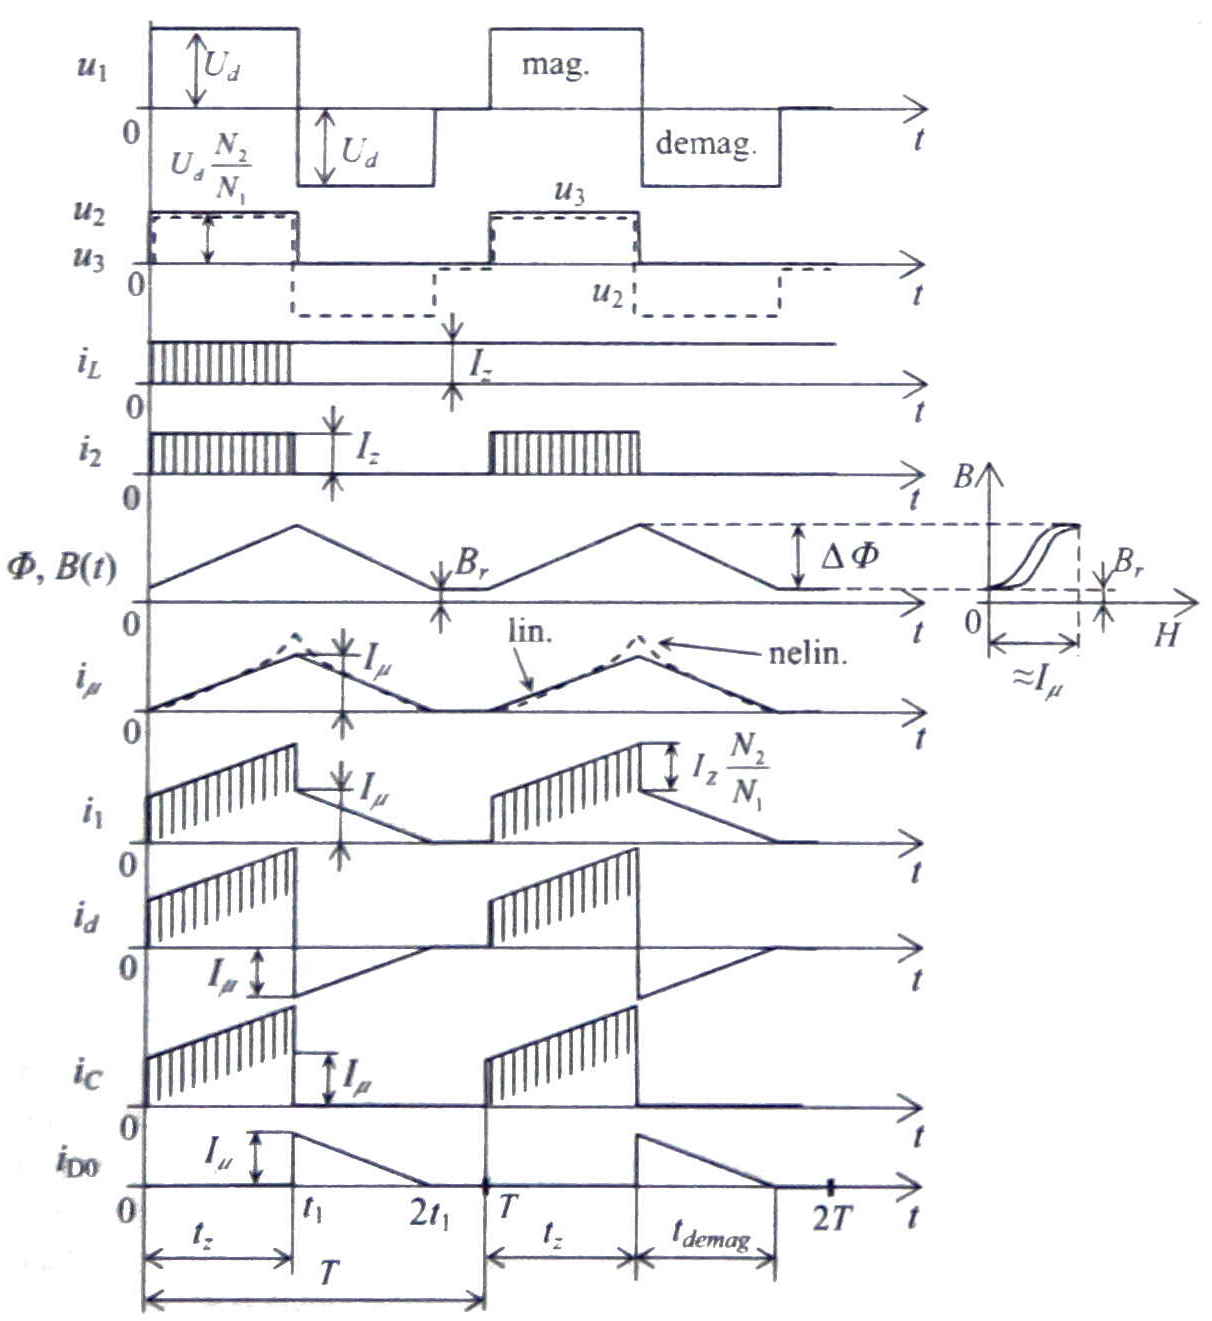
\includegraphics[width=\linewidth]{patocka_1cinprop_menic_w.JPG}
        \caption{Jednočinný propustný měnič - průběhy důležitých veličin.}
        \label{enz:fig_fey_1cinprop_mw} 
      \end{figure}
  
      \begin{figure}
        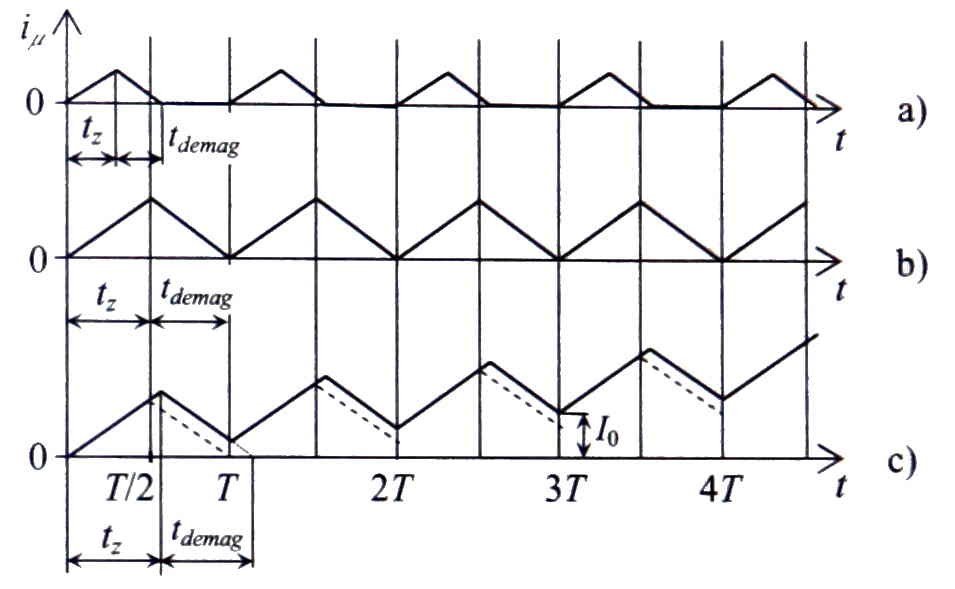
\includegraphics[width=\linewidth]{patocka_1cinprop_syceni.JPG}
        \caption{Demagnetizace transformátoru při různých dobách zapnutí \(t_z\): a) dobrý stav 
                 \(t_z < \frac{T}{2}\), b) mezní stav \(t_z = \frac{T}{2}\), c) špatný stav \(t_z > 
                 \frac{T}{2}\)}.
        \label{enz:fig_fey_1cinprop_syc}
      \end{figure}
      
    %------------- Návrh transformátoru ------------------------------------------------------------
    \subsubsection{Návrh transformátoru}
    
    %------------- Jednočinný propustný měnič s demagnetizačním vinutím ----------------------------
    \subsubsection{Jednočinný propustný měnič s demagnetizačním vinutím}
      \begin{figure}[ht!]
        \centering
        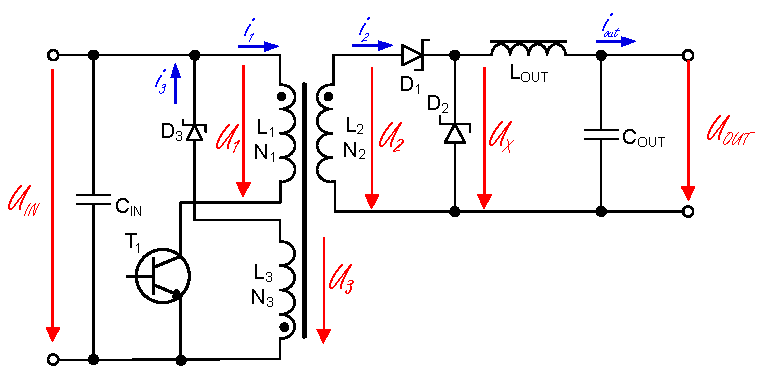
\includegraphics[width=\linewidth]{Forward_converter_topo.pdf}
        \caption[Propustný měnič s akumulační tlumivkou a demagnetizačním vinutím]{Propustný měnič
                 s akumulační tlumivkou  a demagnetizačním vinutím}
        \label{enz:fig_Forward_demag_topo}
      \end{figure}
      
      \newpage
    \subsubsection{Popis činnosti}\label{ENZ:kap_forward_converter_describe}
      Nyní se věnujme podrobnějšímu rozboru funkce propustného měniče. Interval $\delta T$ začíná
      \textbf{sepnutím tranzistoru} $T_1$ kladným impulzem z řídicích obvodů do jeho báze     
      \cite[s.~131]{Hammembauer}, které přivede vstupní napětí na primární vinutí $N_1$. V kapitole
      \ref{ES:kap_rozbor_trafa} byl odvozen vztah \ref{es_eq_int_uprim_max} pro magnetizační tok v 
      jádře transformátoru. Pro nynější případ platí $u_1(t) = U_{in}$. Pak 
      \ref{es_eq_int_uprim_max} nabude tvaru 
      \cite[s.~104]{Patocka}:
      
      \begin{equation}\label{ENZ:eq_forward_phi_mag}
       \Phi_\mu(t)=\frac{1}{N_1}U_{in}t
      \end{equation}
      
      Takže po zapnutí tranzistoru tok lineárně narůstá (z nulové počáteční hodnoty). Na konci doby 
      zapnutí $\delta T$ bude mít své maximum 
      \begin{equation}\label{ENZ:eq_forward_phi_max}
       \Phi_{\mu_{max}}=\frac{1}{N_1}U_{in}\delta T
      \end{equation}
      Během doby $\delta T$ bude sekundární napětí $u_{2}(t)$:
      \begin{equation}\label{ENZ:eq_forward_usec}
       u_{2}(t) = N_2\frac{\Phi_\mu(t)}{dt} = \frac{N_2}{N_1}U_{in} = U_{2}
      \end{equation}
      Čili během doby $\delta T$ je sekundární napětí konstantní. Protože jde o kladné napětí, je 
      $D_1$ otevřená, $D_2$ zavřená a výstupní proud $I_{out}$ musí téci ze sekundárního vinutí 
      transformátoru.
      
      Kolektorovým obvodem a primárním vinutím $N_1$ teče proud $i_{prim}$. Propustně polarizovanou 
      diodou $D_1$ prochází transformovaný vstupní proud přes $L_{out}$ do zátěže a výstupního 
      filtračního kondenzátoru $C_{OUT}$. Tento sekundární proud $i_2$ se časem lineárně zvětšuje od 
      určitého $I_{L_{min}}$ a zároveň se lineárně zvětšuje také proud $i_1$, závislého na převodu 
      transformátoru. Z kapitoly \ref{ES:kap_rozbor_trafa} víme, že primární proud zatíženého 
      transformátoru bude mít hodnotu
      \begin{equation}\label{ENZ:eq_forward_iprim}
      i_1(t) = i_\mu(t) + I_2\frac{N_2}{N_1}
      \end{equation} 
      
      Pro magnetizační proud $i_\mu(t)$ přitom platí vztah (\ref{es_eq_imag_u1}). V našem případě je
      $u_1(t)=U_{in}$ a proto tento vztah dostane konkrétní podobu:
      \begin{equation}\label{ENZ:eq_forward_imagt}
       i_\mu(t) = \frac{U_1t}{L_1}
      \end{equation}
      Vidíme, že stejně jako tok $\Phi_\mu(t)$ tak i magnetizační proud $i_\mu(t)$ lineárně narůstá 
      (z nulové počáteční hodnoty). Na konci $\delta T$ má magnetizační proud své maximum:
      \begin{equation}\label{ENZ:eq_forward_imag_max}
       i_{\mu_{max}}(t) = \frac{U_1\delta T}{L_1}
      \end{equation}
      Během doby $\delta T$ je odebírána energie ze zdroje $U_{in}$ (složka $I_{out}\frac{N2}{N1}$
      primárního proudu) a dodávána do zátěže.
      
      Nyní vypneme tranzistor $T_1$. Proud $i_1(t)$ musí téměř skokem zaniknout. V jádře ale 
      existuje na konci doby $\delta T$ magnetický tok $\Phi_{\mu_{max}}$, odpovídající proudu 
      $I_{\mu_{max}}$. Celková energie magnetického pole v okamžiku vypínání tranzistoru činí 
      $\frac{1}{2}L_1I_{\mu_{max}}$. Proud primárního vinutí je tranzistorem násilně přerušen.
      
      Předpokládejme nejdříve, že neexistuje demagnetizační vinutí $N_3$. Pak by při skokovém zániku
      primárního magnetizačního proudu stejně prudce zanikl i s ním svázaný tok $\Phi_{\mu_{max}}$. 
      Pokles toku s obrovskou (teoreticky nekonečnou) strmostí $-\frac{d\Phi}{dt}$ způsobí vznik 
      napěťového Diracova impulsu, opačné polarity oproti stavu v době $\delta T$, kdy tok narůstal. 
      Tímto impulsem, přičteným k napětí $U_1$, je napěťově namáhán zavírající se tranzistor. Přitom 
      se celá energie $\frac{1}{2}L_1I_{\mu_{max}}$ přemění na křemíkovém čipu v teplo a je příčinou 
      jeho neodvratné destrukce. U reálného tranzistoru je velikost napěťového impulsu vždy omezena 
      průrazným napětím tranzistoru. Nikdy totiž není tranzistor natolik pomalý, že by omezujícím 
      faktorem byla malá strmost $-\frac{di_C}{dt}$ zániku kolektorového proudu během vypínání. 
      Destrukční energetické účinky však zůstávají v každém případě zcela ekvivalentní.              
      
      Aby popsaná situace nenastala, je zde demagnetizační vinutí $N_3$. Děj pak bude vypadat takto: 
      Po vypnutí tranzistoru $T_1$ se opravdu na primárním vinutí objeví napětí $U_1'$ opačné 
      polarity, než bylo $U_1$ v sepnutém stavu, viz. obr. \ref{enz:fig_Forward_demag_wave}. Toto 
      napětí však bude mít přesně definovanou velikost, kterou „dovolí“ vinutí N3. Na tom se totiž 
      objeví také indukované napětí $u_3$. Vzhledem k obrácené orientaci vinutí vůči $N_1$ bude mít 
      záporný pól „na zemi“ a kladný pól na diodě $D_2$. Toto napětí by „chtělo“ být opět teoreticky 
      nekonečné, ale $D_2$ se otevře a pracuje v součinnosti se zdrojem  $U_1$ jako napěťový 
      omezovač, omezující napětí $u_3$ na velikost $U_1$. Celá magnetizační energie 
      $\frac{1}{2}L_1I_{\mu_{max}}$ je vinutím  $N_3$ odevzdána zpět do zdroje. Pak je zřejmé, že 
      napětí indukované v primárním vinutí musí být:
      
      \begin{figure}
        \captionsetup{type=figure}
        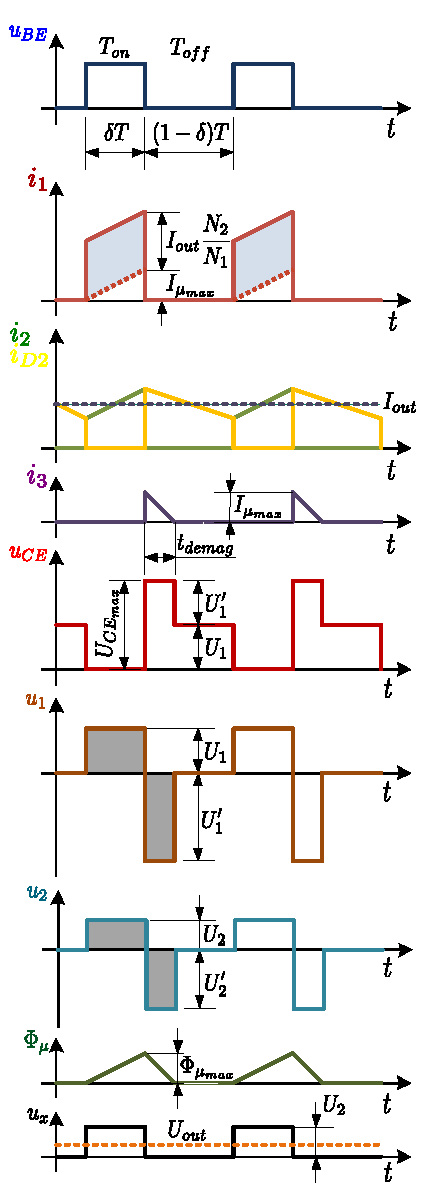
\includegraphics[width=0.9\linewidth]{Forward_converter_wave.pdf}
        \caption{Průběhy veličin propustného měniče s akumulační tlumivkou a demagnetizačním vinutím}
        \label{enz:fig_Forward_demag_wave} 
      \end{figure}                          
      
      \begin{equation}\label{ENZ:eq_forward_u1_demag}
       U_1'=u_3\frac{N_1}{N_3} = U_1\frac{N_1}{N_3}
      \end{equation}
      Tento stav, kdy  $u_1 = -U_1$ a  $u_3 = U_1$, trvá po dobu, než tok $\Phi_\mu(t)$ klesne z 
      počáteční hodnoty $\Phi_{\mu_{max}}$ na nulu. K tomu je třeba konečné doby $t_{demag}$, neboť 
      $U_1$ není nekonečné a proto strmost poklesu $\frac{d\Phi}{dt}$ nemůže být nekonečně velká. 
      Velikost $U_1$ je v této době konstantní a proto klesá tok lineárně. Celý jev se nazývá 
      \emph{demagnetizací jádra}.
      
      Během demagnetizace se předává magnetizační energie jádra zpět do zdroje pomocí proudu 
      $i_3(t)$. Proud $i_3(t)$ je přímo úměrný klesajícímu toku $\Phi_\mu(t)$ takto:
      \begin{equation}\label{ENZ:eq_imag_phi_forward}
       i_3(t) = \frac{1}{L_3}\int{u_3}dt = \frac{1}{L_3}\int{\frac{N_3d\Phi_\mu(t)}{dt}}dt =
       \frac{N_3\Phi_\mu(t)}{L_3}
      \end{equation}
      Po skončení demagnetizace (uplynutí $t_{demag}$) je již magnetický tok nulový, jádro je 
      energeticky neutrální, proto i napětí $u_1$, $u_2$, $u_3$ skokem zanikají na nulu. V 
      neutrálním stavu soustava setrvává až do skončení doby $(1-\delta)T$, tj. do zapnutí 
      tranzistoru.
      
      Pro magnetický tok během procesu demagnetizace musí platit:
      \begin{equation}\label{ENZ:eq_phi_mag_forward}
       \Phi_\mu(t) = \Phi_{\mu_{max}} - \frac{\int{u_1(t)dt}}{N_1} = \Phi_{\mu_{max}} -
       \frac{U_1't}{N_1}
      \end{equation}
      Po uplynutí $t_{demag}$ je tok nulový. Položíme-li tedy $\Phi_\mu(t)$ dle
      (\ref{ENZ:eq_phi_mag_forward}) rovný nule, lze odsud vyjádřit $t_{demag}$.
      \begin{equation}\label{ENZ:eq_tdemag_forward}
       t_{demag} = \frac{N_1\Phi_{\mu_{max}}}{U_1'}
      \end{equation}
      Za $\Phi_{\mu_{max}}$ dosadíme vztah (\ref{ENZ:eq_forward_phi_max}) a za $U_1$  vztah
      (\ref{ENZ:eq_forward_u1_demag}). Tím dostaneme:
      \begin{equation}\label{ENZ:eq_tdemag_N1N3_forward}
       t_{demag} = \frac{N_3}{N_1}\delta T
      \end{equation}
      Je zřejmé, že musíme zajistit, aby $(1-\delta)T > t_{demag}$, jinak by tok ještě nestačil
      úplně zaniknout a už bychom znovu spínali tranzistor. V průběhu dalšího sepnutí by se tok (a
      magnetizační proud) zvýšil opět o hodnotu $\Phi_{\mu_{max}}$ (resp.  $I_{\mu_{max}}$, ale už z
      nenulové počáteční hodnoty a tak by neustále vzrůstal (během dalších period by se
      „naintegroval“ teoreticky na hodnotu $\rightarrow\infty$), až by došlo k přesycení jádra a tím
      k prudkému lavinovitému růstu magnetizačního proudu (neboť by současné klesla indukčnost
      $L_1$). Jev by postupoval až do zničení tranzistoru. Z výše uvedeného důvodu musí být
      maximální střída $\delta$ omezena na hodnotu:
      \begin{equation}\label{ENZ:eq_forward_delta_max}
      \delta_{max} = \frac{t_{on}}{t_{on}+t_{demag}}
      \end{equation}
      Dosazením (\ref{ENZ:eq_tdemag_N1N3_forward}) za $t_{demag}$ dostaneme:
      \begin{equation}\label{ENZ:eq_forward_delta_max1}
      \delta_{max} = \frac{N_1}{N_1+N_3}
      \end{equation}
      Výstupní napětí $U_{out}$ je rovno \emph{střední hodnotě napětí} $u_X$ a platí proto:
      \begin{equation}\label{ENZ:eq_uout_forward_delta}
      U_{out} = U_1\frac{N_2}{N_1}\frac{t_{on}}{t_{on} + t_{off}} = U_1\frac{N_2}{N_1}\delta
      \end{equation}
      
     %---------- Proudové a napěťové dimenzování součástek -----------------------------------------
    \subsubsection{Proudové a napěťové dimenzování součástek}
      V době $t_{demag}$ je tranzistor namáhán napětím $U_{{CE}_{max}}$:
      \begin{equation}\label{ENZ:eq_dim_Ucemax}
        U_{{CE}_{max}} = U_1 + U_1' = U_1 + \frac{N_3}{N_1}U_1 = U_1\frac{N_1+N_3}{N_1}
      \end{equation}
      \begin{itemize}
       \item Volíme-li $N_3 < N_1$, je $U_1' > U_1$ a tedy namáhání $U_{{CE}_{max}} > 2U_1$. Zato
             je ale maximální dovolená střída $\delta_{max} > 0,5$ a je tedy větší maximální
             dosažitelné výstupní napětí.
       \item Volíme-li $N_3 > N_1$, je $U_1' < U_1$ a je tedy  $U_1 < U_{{CE}_{max}} < 2U_1$. Zato
             je ale maximální dovolená střída $\delta_{max} < 0,5$ a je tedy menší maximální
             dosažitelné výstupní napětí.
      \end{itemize}
      Volba  poměru  $N_3/N_1$ proto záleží na tom, co je v dané aplikaci více kritické, zda
      napěťové namáhání tranzistoru,  či co největší dosažitelné výstupní napětí (s neměnným
      převodem  $N_2/N_1$). V praxi se nejčastěji volí $N_3 = N_1$ z důvodů snadného souběžného
      (\emph{bifilárního}) vinutí obou cívek - viz později.
      
      \begin{itemize}
        \item \emph{Proudové a dimenzování $T_1$:}
           \newline Zanedbáme-li magnetizační proud, pak lze psát, viz. obr.
           \ref{enz:fig_Forward_demag_wave}, pro špičkovou, střední a efektivní hodnotu
           kolektorového proudu tranzistoru následující rovnice:
            \begin{align}
                I_{1_{max}} &= I_{out}\frac{N_2}{N_1}             \\
                I_{1_{av}}  &= I_{out}\frac{N_2}{N_1}\delta       \\
                I_{1_{rms}} &= I_{out}\frac{N_2}{N_1}\sqrt{\delta}
            \end{align}
        \item \emph{Proudové a napěťové dimenzování $D_1$:}
            \begin{align}
                I_{D_{1max}} &= I_{out}                \\
                I_{D_{1av}}  &= I_{out}\delta          \\
                I_{D_{1rms}} &= I_{out}\sqrt{\delta}   \\
                U_{D_{1Rmax}}&= U_1\frac{N_2}{N_3}
            \end{align}
        \item \emph{Proudové a napěťové dimenzování $D_2$:}
            \begin{align}
                I_{D_{2max}} &= I_{out}                \\
                I_{D_{2av}}  &= I_{out}(1-\delta)      \\
                I_{D_{2rms}} &= I_{out}\sqrt{1-\delta} \\
                U_{D_{2Rmax}}&= U_1\frac{N_2}{N_1}
            \end{align}
        \item \emph{Proudové a napěťové dimenzování $D_3$:}
            \begin{align}
                I_{D_{3max}} &= I_3        = I_{\mu_{max}}\frac{N_1}{N_3} =
                                             \frac{U_1\delta_{max}T}{L_1}\cdot\frac{N_1}{N_3}   \\
                I_{D_{3av}}  &= I_{3_{av}} = \frac{I_3}{2}\delta                                \\
                I_{D_{3rms}} &=  \sqrt{\frac{1}{T}\int_0^{t_{demag}}
                                {\left(I_3\frac{t}{t_{demag}}\right)^2}dt} =
                                 \frac{I_3}{\sqrt{3}}\sqrt{\frac{t_{demag}}{T}}                 \\
                U_{D_{3Rmax}}&= U_1 + U_1\frac{N_3}{N_1}
            \end{align}
      \end{itemize}
      \begin{note}
        Všimneme si, že funkce tohoto měniče je kromě transformátoru zcela analogická funkci
        snižujícího měniče z kap. \ref{ENZ:kap_step_down}. Horní spínač je zde rozdělen tak, že
        tranzistor je na primární straně (pro větší podobnost s obr. \ref{enz:fig_StepDown_sch1}
        lze v obr. \ref{enz:fig_Forward_demag_topo} vzájemně zaměnit umístění tranzistoru a        
        primárního vinutí transformátoru, tj. z kladného pólu $U_{in}$ nejprve tranzistor). Dioda
        $D_2$, tvořící s tranzistorem horní spínač, je až na sekundární straně. Dioda $D_1$ jen
        odděluje výstupní obvod od sekundárního napětí v době, kdy je záporné, protože  toto napětí
        nemůže mít nenulovou stejnosměrnou složku (stejně tak ani napětí $u_1$ a $u_3$).
      \end{note}
  
    \subsubsection{Přehled metod demagnetizace jádra transformátoru}
      V kapitole \ref{ENZ:kap_forward_converter_describe} byl popsán jeden z možných způsobů, jak
      demagnetizovat jádro transformátoru, tak aby v dalším pracovním cyklu nedošlo k posunu
      pracovního bodu magnetického materiálu jádra a následně k jeho přesycení. Velikost
      magnetizačního proudu je dle vztahu \ref{ENZ:eq_forward_imag_max} dána poměrem napěťové plochy
      $U_{in}\cdot t_{on}$ přiložené na vinutí primární cívky a hodnotou její magnetizační
      indukčnosti ($L_{mag} = L_{1}$) $$i_{mag} = \frac{U_{prim}\cdot{t_{on}}}{L_{mag}}$$.
      
      \begin{figure}[ht!]
       \centering
       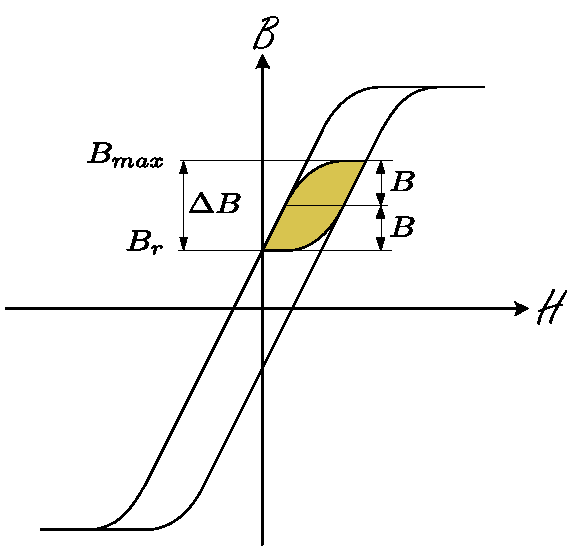
\includegraphics[width=0.4\textwidth]{BH_curve_forward_converter.pdf}
       \caption[Hysterezní smyčka]{Transformátor jednočinného propustného měniče pracuje v prvním
                kvadrantu hysterezní smyčky}
       \label{enz:fig_Forward_Hyst_loop}
      \end{figure}  
      
      Pracovní oblast transformátoru je v prvním kvadrantu, jak naznačuje obr.
      \ref{enz:fig_Forward_Hyst_loop}, neboť polovodičový spínač přikládá mezi svorky primárního
      vinutí pouze unipolární pulzy. Měnič se také proto nazývá \emph{jednočinný}, protože energie je
      ze zdroje předávána do zátěže pouze jedenkrát za periodu, v jednom tzv. aktivním běhu, tj. v
      době $t_{on}$, kdy je tranzistor sepnut a magnetická indukce se v jádře zvyšuje z hodnoty
      remanentní indukce $B_r$ o velikost magnetického zdvihu $\Delta B$.
      
      \begin{figure}[ht!]
      \centering
      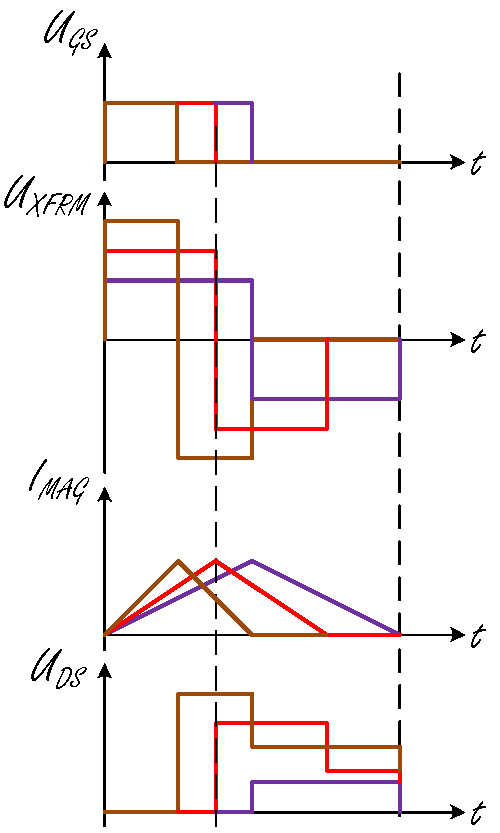
\includegraphics[width=0.4\textwidth]{imag_forward_converter.pdf}
      \caption[Magnetizační proud]{Vrcholová hodnota magnetizačního proudu je konstantní pro
               jakékoliv velikosti vstupního napětí, neboť regulační smyčka zajistí, aby napěťová
               plocha $V_{in}\cdot t_{on}$ byla konstantní}
      \label{enz:fig_imag_forward_converter}
      \end{figure}
      
      Pokud bychom měřili magnetizační proud primárního vinutí, dospěli bychom k průběhům na obr.
      \ref{enz:fig_imag_forward_converter}, jenž vykazují stejnou vrcholovou hodnotu pro různé hodnoty
      vstupního napětí. Je to dáno tím, že pokud měnič během měření pracoval v uzavřené regulační
      smyčce, bude součin $V_{in}\cdot t_{on}$ konstantní a za předpokladu, že magnetizační indukčnost
      je též neměnná, pak dle předchozí rovnice dospějeme $i_{mag_{max}} = konst$.
     
      %------------- Jednočinný propustný měnič s aktivním clampingem ------------------------------
    \subsubsection{Jednočinný propustný měnič s aktivním clampingem}\label{ENZ:kap_afwdconv}  
      \begin{figure*}[ht!]
        \centering
        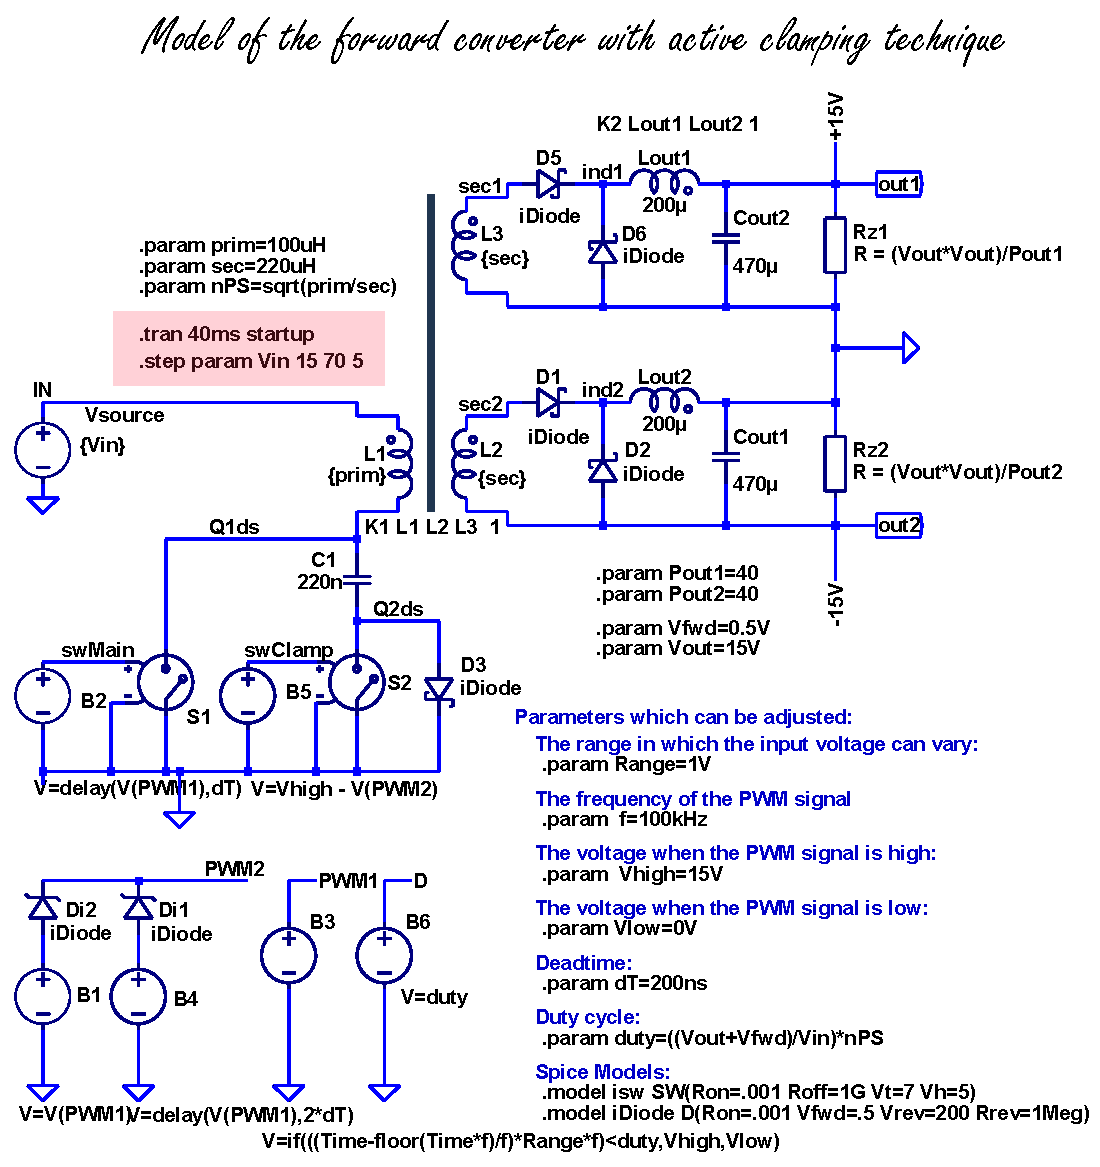
\includegraphics[width=0.7\textwidth]{forward_converter_active_ltspice_model.pdf}
        \caption[Propustný měnič s aktivním clampingem]{Propustný měnič s aktivním clampingem}
        \label{enz:fig_imag_a_lt_frwd_conv}
      \end{figure*}   
      
    \subsubsection{Vlastnosti měniče}
      Obecně pro všechny varianty  propustných měničů s transformátorem lze říci, že jsou vhodné pro
      přenos velkých výkonu. Je to dáno principem činnosti, kdy proud podílející se na přenosu výkonu
      se nepodílí na magnetizaci jádra transformátoru (teče v době $t_{on}$ a to jak na sekundární
      straně tak i na primární – kompenzace magnetických účinku). Může se proto zvyšovat, aniž by
      rostlo sycení jádra transformátoru. Toto sycení je určeno pouze integrálem primárního napětí a
      počtem primárních závitu. Lze proto zvýšením pracovního kmitočtu docílit zmenšení velikosti
      transformátoru, jak to bylo vysvětleno na konci kap. \ref{ES:kap_simple_rozbor_trafa}.
 
  \subsection{Jednočinný blokující měnič}
    Základem tohoto měniče je „invertující měnič se společnou tlumivkou“ z kapitoly
    \ref{ENZ:kap_buck_boost}. Všimneme si, že z původního schématu (obr. 8.12) vymizela tlumivka,
    jejíž funkci nyní zastane transformátor. Princip činnosti je vlastně úplně stejný, pokud si
    uvědomíme, že jádro nynějšího transformátoru je magnetováno stejně jako jádro tlumivky na obr. 
    8.12, viz. průběh $i_L(t)$ v obr. 8.12 a průběh $\Phi_\mu(t)$ v obr.9.8. Jediný rozdíl je v tom, 
    že stejných magnetických poměrů je nyní dosaženo pomocí dvou vinutí místo původního jednoho (v 
    době $t_1$ pomocí $L_1$ a v době $t_2$ pomocí $L_2$). Tím se dosáhne galvanického oddělení. 
    Vznikl tak transformátor, ovšem režim jeho činnosti je takový, že magnetické účinky v jádře se 
    podobají tlumivce. Režim je zcela odlišný od režimu transformátoru v propustných měničích.

    %------------------------------------------------------
    %------------------------------------------------------
    % Section: Metody regulace spínanich zdrojů
      % file: Control_Techniques.tex
%============================= Podkapitola: Metody regulace spínaných zdrojů =======================
\section{Metody regulace spínaných zdrojů}
      \subsection{Základy impulzní regulace}
        Základním principem a současně odlišností impulsní regulace od regulace klasické je její
        nespojitost. To v zásadě znamená, že nehledě na detailní realizaci, je výstupní napětí
        $U_out$ stabilizováno zásahy regulačního členu pouze v určitých, časově omezených
        intervalech $T_a$. \cite{Hammembauer}

        Srovnejme pro názornost klasický a impulsní regulátor na úrovni blokových schémat. (obr.
        4.1 a obr. 5.9 ). Vidíme, že obě jsou formálně dosti podobná. U obou nacházíme napěťový
        normál $U_{REF}$, zesilovač regulační odchylky $A_u$, budící obvod i výkonový regulační
        člen a samozřejmě i zpětnovazební smyčku. Tím však, snad až na základní podstatu regulační
        smyčky podobnost končí. Funkčně jsou oba regulátory naprosto odlišné.

        U spojitého lineárního regulátoru ovládá odchylka výstupního napětí od jmenovité velikosti
        spojitě okamžitý odpor výkonového regulačního členu v libovolném okamžiku tak, aby výstupní
        napětí bylo konstantní.

      \subsection{Regulační smyčka}

      \subsubsection{Porovnání regulátoru s napěťovým a proudovým řízením}
        \begin{figure*}
          \centering
          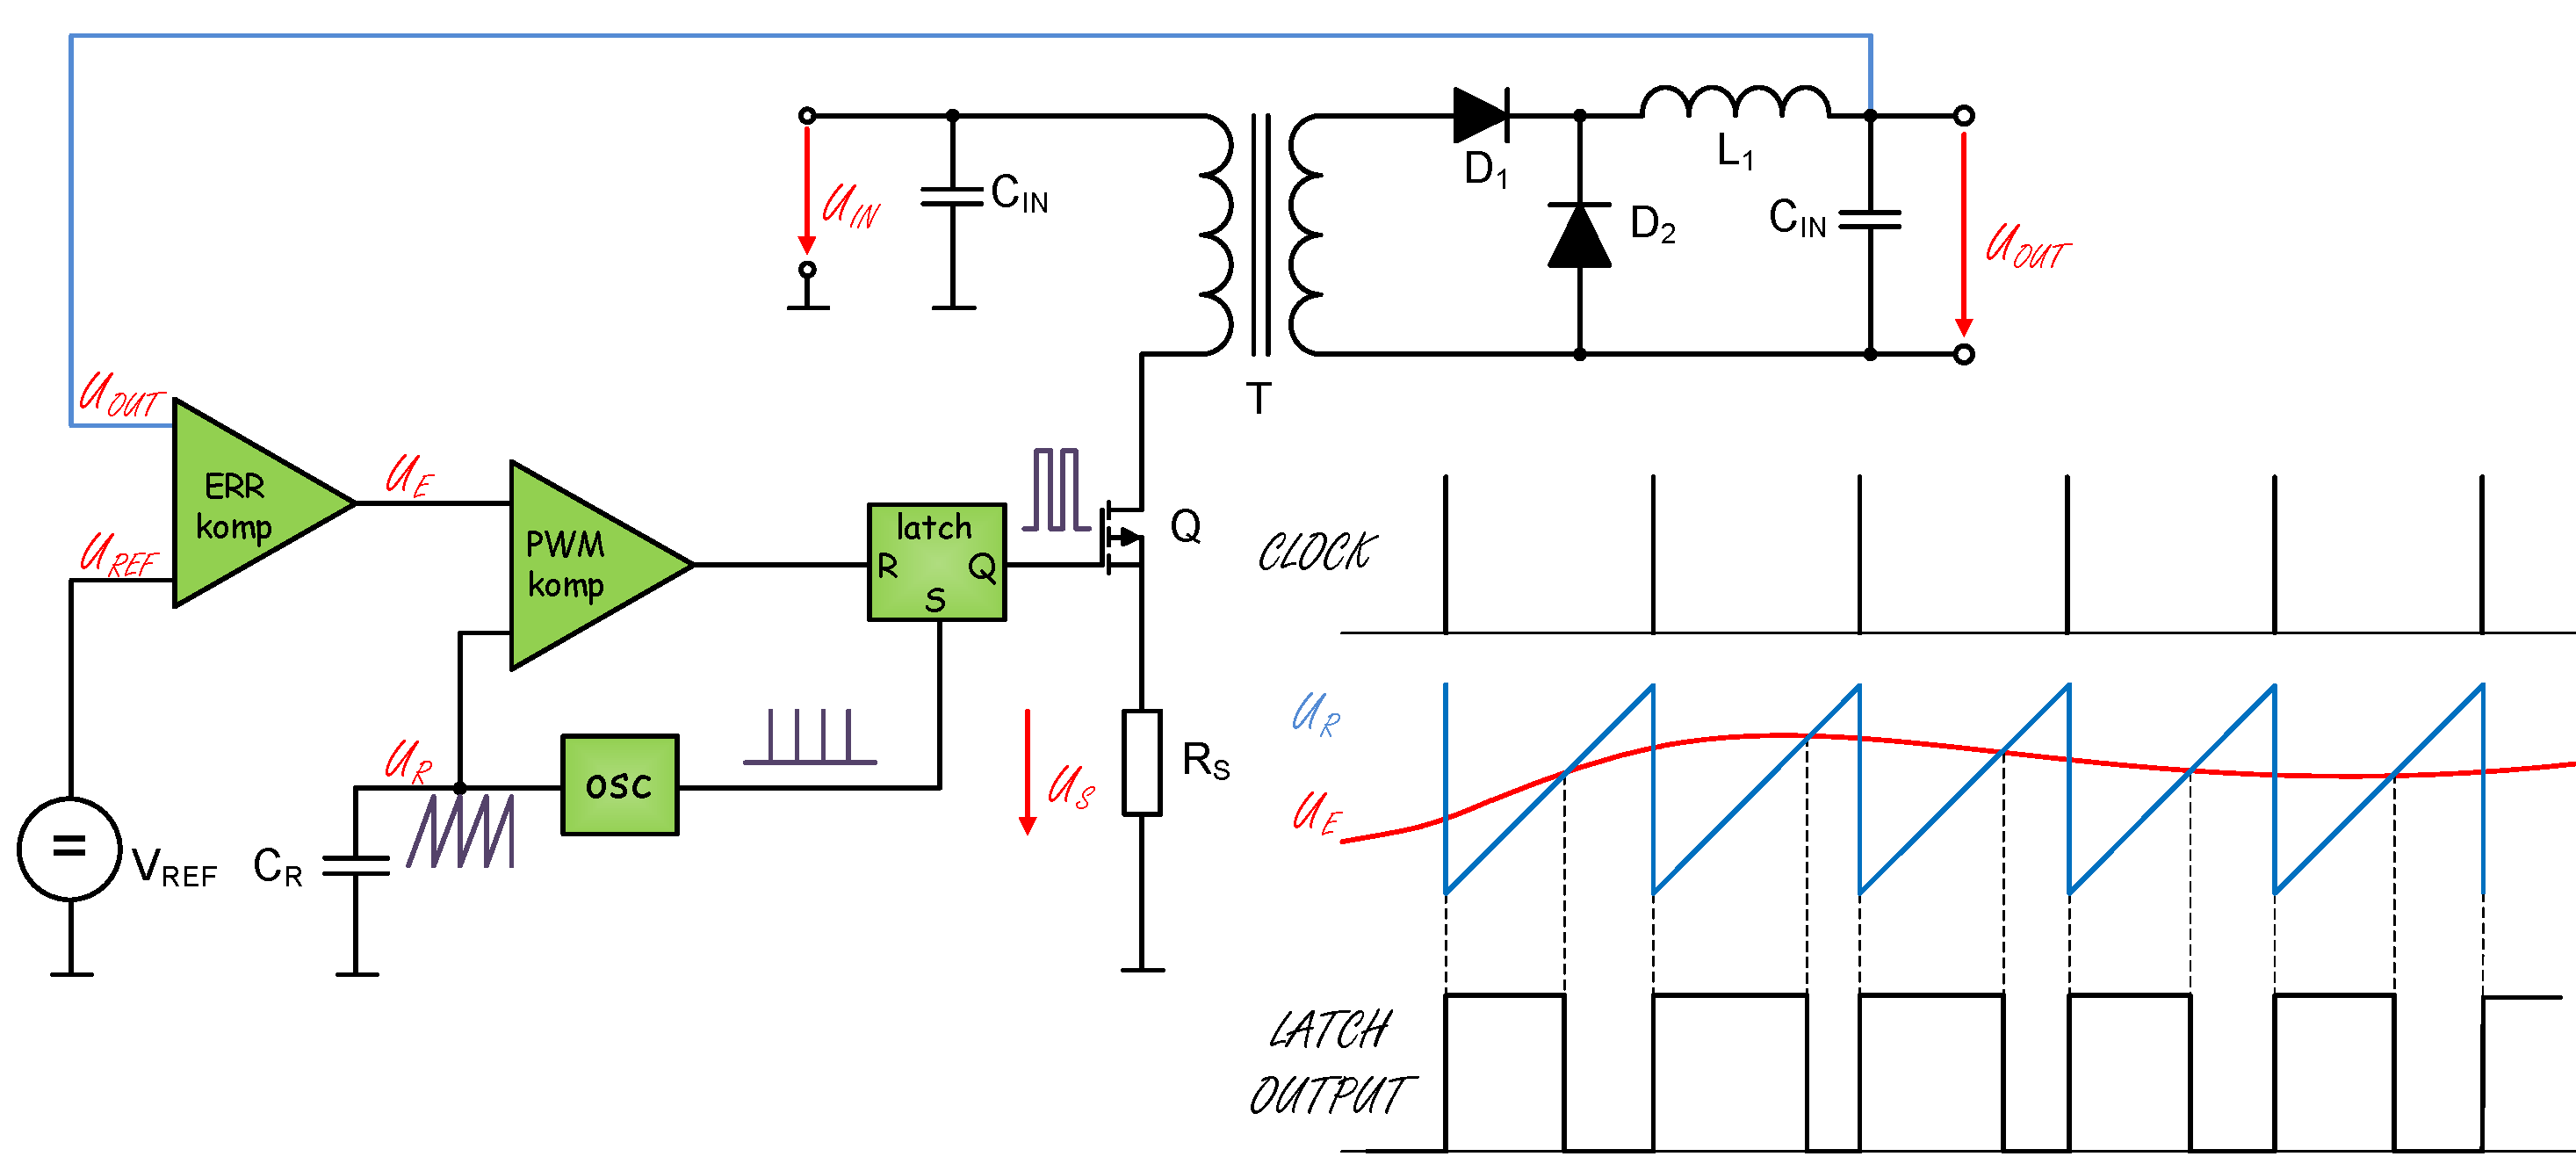
\includegraphics[width=0.6\textwidth]{unitrode_voltage_mode_control.pdf}
          \caption[Regulátor s napěťovým řízením]{Regulátor s napěťovým řízením - Voltage mode
                   control [\cite{SLUA119}]}
          \label{ENZ:fig_V_mode_cntrl}
        \end{figure*}

         The current mode control method uses two control loops --an inner, current control loop
         and an outer loop for voltage control. Figure  1 shows a forward converter (buck family)
         using current mode control. When the switching transistor is on, current through Rsense is
         proportional to the upward ramping filter inductor current. When the ramp voltage Vs
         reaches Ve (the amplified  output  voltage  error), the switching transistor turns  off.
         Thus, the outer voltage control loop defines the level at which the inner loop regulates
         peak current through the switch and through the filter inductor. \cite{SLUP075}

        \begin{figure*}
          \centering
          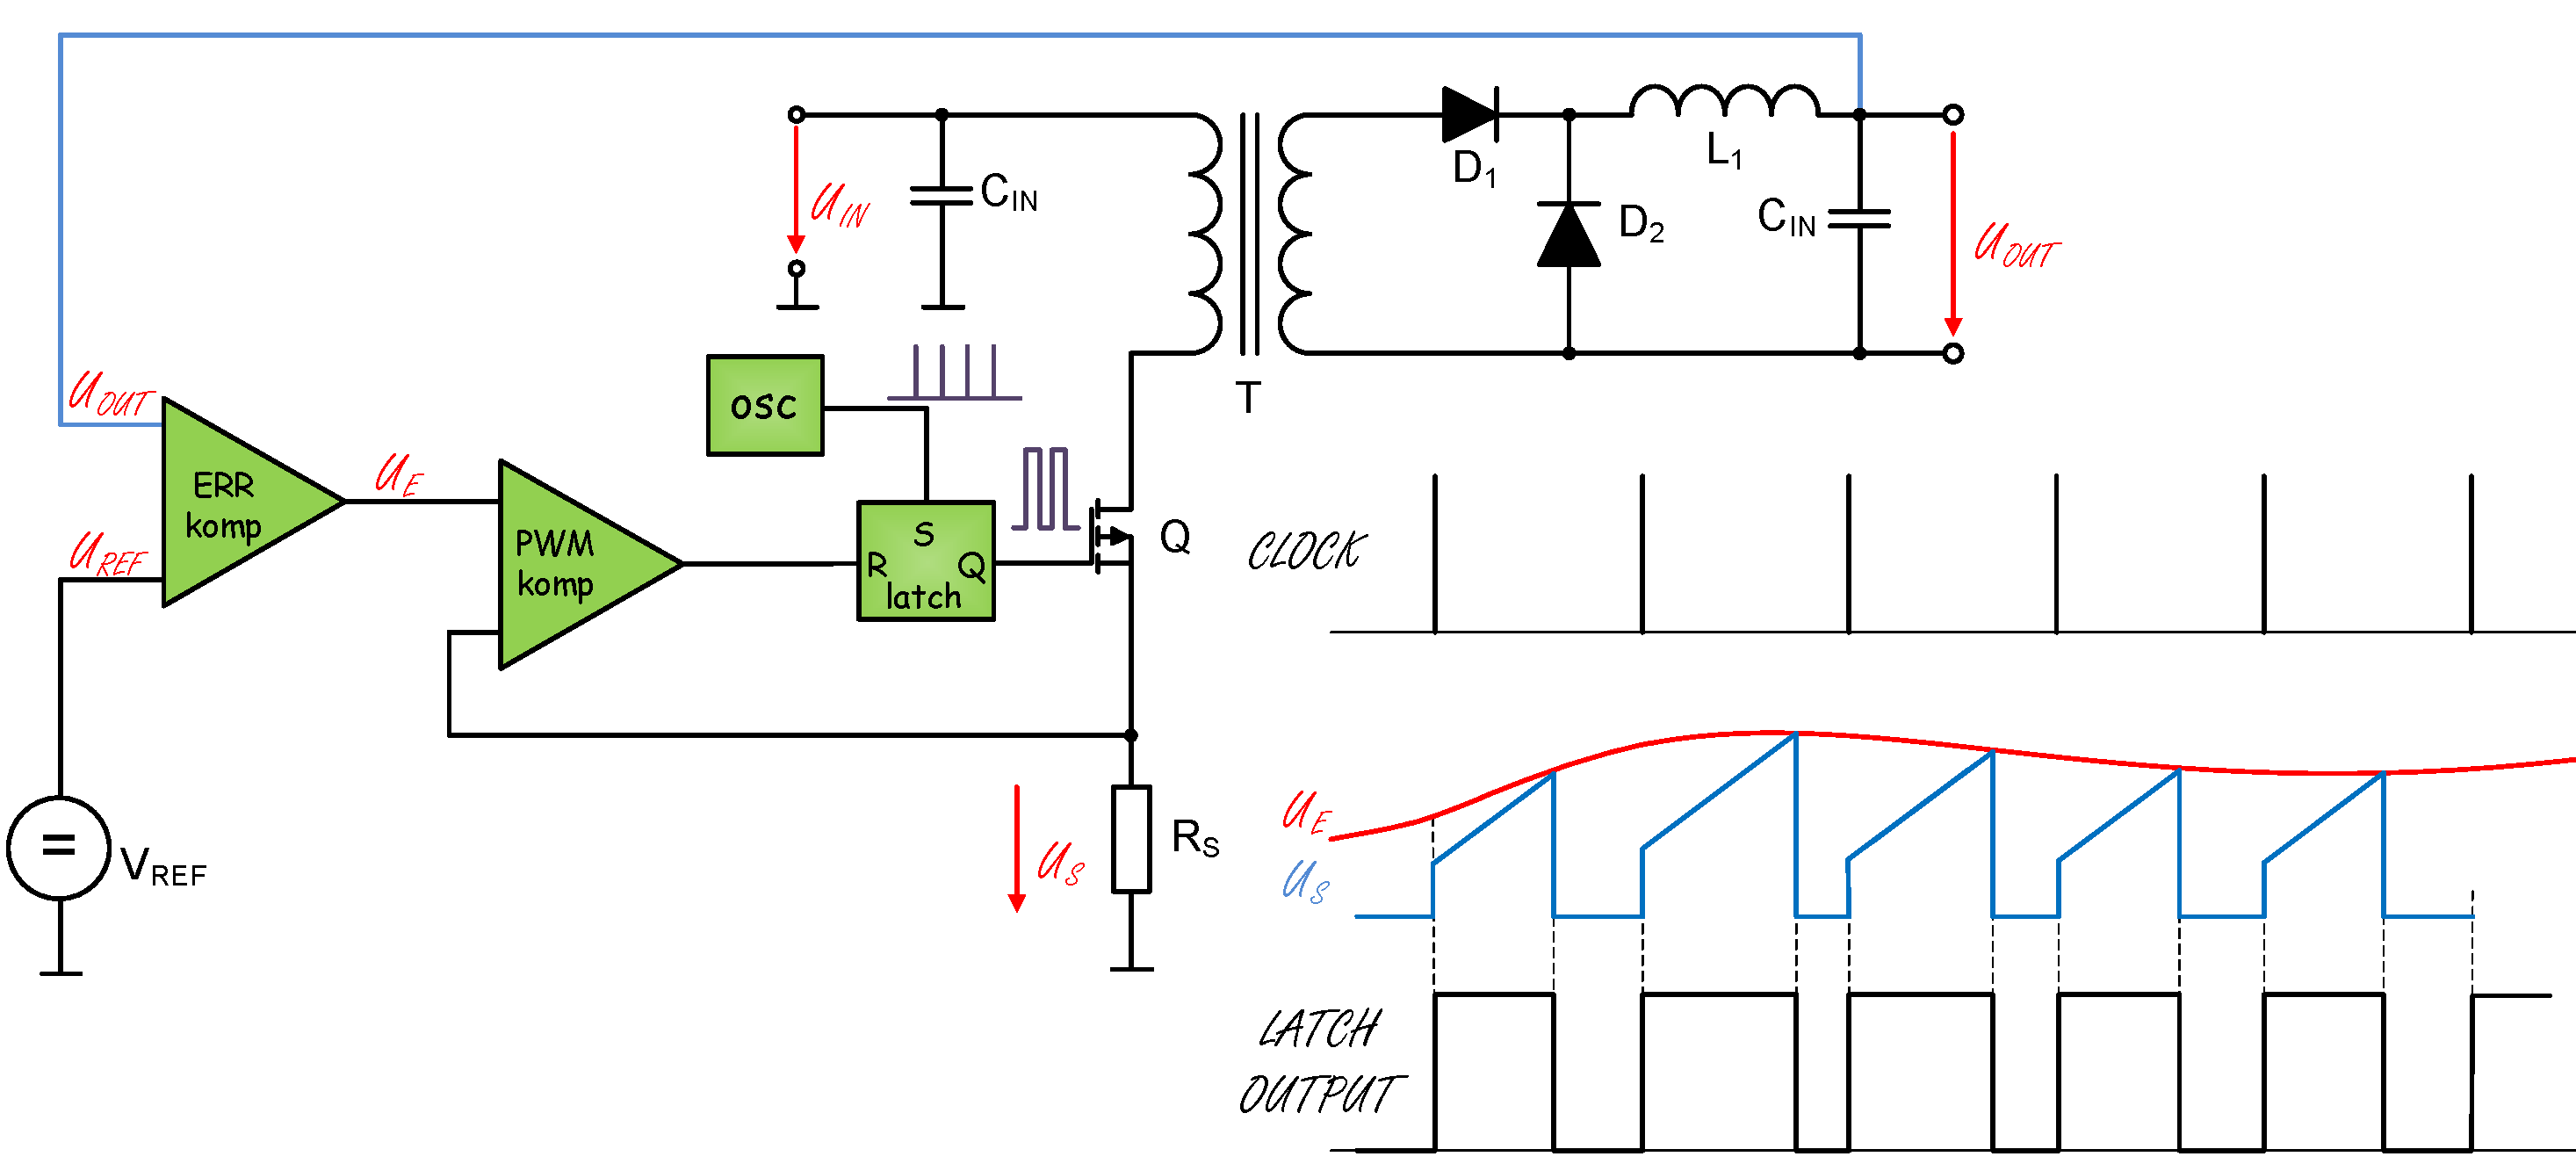
\includegraphics[width=0.6\textwidth]{unitrode_current_mode_control.pdf}
          \caption[Regulátor s proudovým řízením]{Regulátor s proudovým řízením - Current mode
                   control [\cite{SLUA119}]}
          \label{ENZ:fig_I_mode_cntrl}
        \end{figure*}

        Výhody:
        \begin{itemize}
          \item Input voltage feed-forward, resulting in good open-loop line regulation.
          \item Simplified loop --inductor pole and 2nd order characteristic eliminated.
          \item Optimum large-signal behavior.
          \item No conditional loop stability  problems.
          \item Flux balancing (symmetry correction) in push-pull circuits.
          \item Automatic pulse-by-pulse current limiting.
          \item Current sharing of paralleled supplies for modular power systems.
          \item Less complexity/cost (current sense/amp is not an added complication).
        \end{itemize}

        Nevýhody (continuous  mode  only):
        \begin{itemize}
          \item Peak/avg. current error and instability --slope compensation
          \item Noise immunity is  worse because of  shallower ramp.
          \item Half Bridge runaway
          \item DC open loop load regulation is worse.
          \item (1-D) current error in Boost or Flyback circuits.
          \item Loop irregularities with multiple output buck circuits.
        \end{itemize}

    %------------------------------------------------------

  \section{Sbírka katalogových zapojení neizolo\-va\-ných měničů}
    Existují dvě možnosti, jak provádět řízení pomocí PWM odlišující se \emph{typem zpětné
    vazby}, která je buď čistě \textbf{napěťovou vazbou} (\emph{voltage mode control}), nebo
    \emph{napěťovou vazbou s vnitřní proudovou smyčkou} (\emph{current mode control}). V
    následující diskusi se pokusíme konzistentním způsobem vysvětlit vlastnosti obou řídících
    algoritmů (slua119)
    
    \subsection{Zdroj symetrického napětí s jedním induktorem}
      \begin{figure}
        \centering
        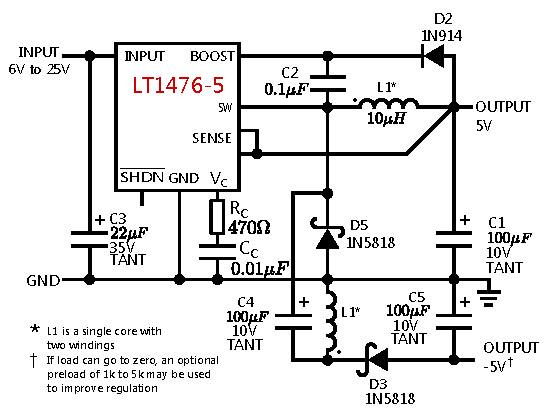
\includegraphics[width=\linewidth]{LT1376_dual_output_reg.pdf}
        \caption[Spínaný zdroj napětí $\pm5 V$ vystačí s jedinou indukčností s dvojím
                 vinutím]{Spínaný zdroj napětí $\pm5 V$ vystačí s jedinou indukčností s dvojím
                 vinutím. \cite{DN100}. Linear Technology Corp. (Dual Output Regulator Uses Only
                 One Inductor)}
        \label{enz:fig_LT1376_cir1}
      \end{figure}
      Toto řešení na obr. \ref{enz:fig_LT1376_cir1} nabízí spínaný zdroj symetrického napětí za
      použití několika dalších součástek a induktoru s dvojím vinutím. Základní části zdroje je
      napěťový regulátor snižující vstupní kladné napětí založený na obvodu \emph{LT1376-5} se
      spínacím kmitočtem 500 kHz a možností zatížení proudem až 1,5 A.

      \begin{figure}
        \centering
        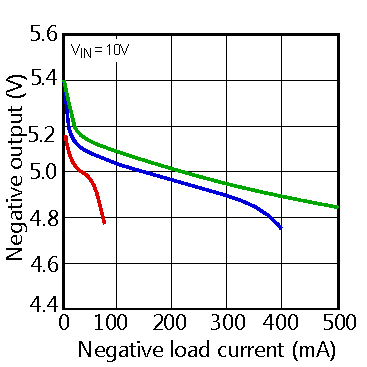
\includegraphics[width=\linewidth]{LT1376_dual_output_reg_performance.pdf}
        \caption{Zatěžovací charakteristika záporné větve.}
        \label{enz:fig_LT1376_cir1_perform}
      \end{figure}

      Druhá polovina induktoru $L_1$ společně s $D_3$, $C_5$ a $C_4$ je určena pro tvorbu
      záporného napětí pomocí \textbf{SEPIC topologie} - \emph{Single Ended Primary Inductance
      Converter}. Kondenzátor $C_4$ vnucuje oběma vinutím stejné napětí. Bez něho pracuje tato
      část jako blokující měnič (\textbf{flyback}), která by sice poskytla -5V, ale jen naprázdno
      se značnou závislostí na zátěži (nedokonalá vazba mezi vinutími).
